\documentclass[letterpaper, 11pt, oneside]{article}
% idioma
\usepackage[utf8]{inputenc} %Para configuración de caracteres
\usepackage[spanish]{babel} %Para configuración de idioma
\pretolerance=20000
\tolerance=30000

\usepackage{enumitem}

\usepackage{array}

%tablas
\usepackage{booktabs}
%rotar tablas
\usepackage{rotating}
%color tablas
\usepackage{colortbl}

% \usepackage[numbib,notlof,notlot,nottoc]{tocbibind} %Para que la biliografía se llame así y no referencias y para que quede numerada como sección.
%\usepackage[notlof,notlot,nottoc]{tocbibind} %Bibliografía sin numerar
\bibliographystyle{ieeetr} %Estilo de bibliografía IEEE

%VARG: Para poder colocar texto en color
\usepackage{color}
\definecolor{naranja}{rgb}{1,0.5,0} % valores de las componentes roja, verde y azul (RGB)
\definecolor{rojo}{rgb}{1,0,0}

%VARG: Para tener los bookmarks del pdf (menú al lado derecho en los visualizadores de pdf)
% si colorlinks= true, no salen las cajas, sino el color del link!!
% linkcolor para los indices, citecolor para las citas en texto, urlcolor para los enlaces
\usepackage[pdftex,bookmarks=true, linkcolor=black, citecolor=black, colorlinks=true, urlcolor=black]{hyperref}

%VARG: Para poder hacer subfiguras (subfloat)
\usepackage{subfig}

%espaciado
 \usepackage{setspace}
 \onehalfspacing
 \setlength{\parindent}{0pt}
%  \setlength{\parskip}{2.0ex plus0.5ex minus0.2ex}

%margenes según  icontec
\usepackage{vmargin}
\setmarginsrb           { 4.0cm}  % left margin
                        { 4.0cm}  % top margcm
                        { 2.0cm}  % right margcm
                        { 3.0cm}  % bottom margcm
                        {  10pt}  % head height
                        {0.25cm}  % head sep
                        {   9pt}  % foot height
                        { 1.0cm}  % foot sep

% inserción url's notas de pie.
\usepackage{url}

% Paquetes de la AMS:
\usepackage{amsmath, amsthm, amsfonts}

% Teoremas
%--------------------------------------------------------------------------
\newtheorem{thm}{Teorema}[section]
\newtheorem{cor}[thm]{Corolario}
\newtheorem{lem}[thm]{Lema}
\newtheorem{prop}[thm]{Proposición}
\theoremstyle{definition}
\newtheorem{defn}[thm]{Definición}
\theoremstyle{remark}
\newtheorem{rem}[thm]{Observación}

% Atajos.
% Se pueden definir comandos nuevos para acortar cosas que se usan
% frecuentemente. Como ejemplo, aqu se definen la R y la Z dobles que
% suelen representar a los conjuntos de nmeros reales y enteros.
%--------------------------------------------------------------------------

\def\RR{\mathbb{R}}
\def\ZZ{\mathbb{Z}}

% De la misma forma se pueden definir comandos con argumentos. Por
% ejemplo, aqu definimos un comando para escribir el valor absoluto
% de algo ms fcilmente.
%--------------------------------------------------------------------------
\newcommand{\abs}[1]{\left\vert#1\right\vert}

% Operadores.
% Los operadores nuevos deben definirse como tales para que aparezcan
% correctamente. Como ejemplo definimos en jacobiano:
%--------------------------------------------------------------------------
\DeclareMathOperator{\Jac}{Jac}


\newcommand\portada{
\begin{titlepage}
		\begin{center}
			{\large \bf OBJETO VIRTUAL DE APRENDIZAJE PARA LA TEORÍA DEL CAOS Y SU RELACIÓN CON LOS FRACTALES}
			\vfill
% 			{\large\bf PRESENTADO POR \par}
			{\large\bf ANDRÉS RICARDO TORRES MARTÍNEZ\par}
			{\large\bf aritoma@gmail.com\par}
			\vfill
			{\large\bf UNIVERSIDAD DEL VALLE  \par}
			{\large\bf FACULTAD DE INGENIERÍA \par}
			{\large\bf ESCUELA DE INGENIERÍA DE SISTEMAS Y COMPUTACIÓN \par}
			{\large\bf SANTIAGO DE CALI \par}
			{\large\bf ENERO 2011 \par}
		\end{center}
\end{titlepage}
}

\newcommand\contraportada{
	\begin{titlepage}
		\begin{center}
			{\large \bf OBJETO VIRTUAL DE APRENDIZAJE PARA LA TEORÍA DEL CAOS Y SU RELACIÓN CON LOS FRACTALES } 
			\vfill
			{\large\bf ANDRÉS RICARDO TORRES MARTÍNEZ}
			\vfill
			{\large\bf Código 0439549 \par}
			
			\vfill
			{Director \par}
			{\bf Ing. Angel García Baños, Ph.D. \par}
			{Profesor de la Escuela de Ingeniería de Sistemas y Computación \par}
			\vfill
			{\large\bf UNIVERSIDAD DEL VALLE \par}
			{\large\bf FACULTAD DE INGENIERÍA \par}
			{\large\bf ESCUELA DE INGENIERÍA DE SISTEMAS Y COMPUTACIÓN \par}
			{\large\bf SANTIAGO DE CALI \par}
			{\large\bf ENERO 2011 \par}
		\end{center}
\end{titlepage}
}

\begin{document}
\portada
\contraportada

\renewcommand\contentsname{\centering Índice}
\tableofcontents
\clearpage

\renewcommand\listfigurename{\centering Índice de imagenes}
\listoffigures
% \clearpage

\renewcommand\listtablename{\centering Índice de tablas} 
\listoftables
\clearpage



\begin{center}
 \section{Introducción}
\end{center}
La educación se encuentra en la búsqueda de mejores alternativas de sistemas de enseñanza aprovechando la evolución continua de la tecnología, dando a los educadores más herramientas para lograr el gusto por aprender y mejorar el desarrollo creativo e imaginativo de sus alumnos. \\

El aprendizaje por medio de un sistema informático está alcanzando niveles importantes de difusión y aceptación. Sin embargo, el desarrollo de aplicaciones y herramientas que contribuyen a fortalecer procesos de enseñanza  se realiza frecuentemente de manera intuitiva, es decir, sin un análisis detallado de los factores que intervienen en dichos procesos, esta situación limita notablemente la incidencia de la tecnología en la educación. \\

La informática y pedagogía han madurado lo suficiente para enriquecer los ambientes educativos con novedosas propuestas. Esto permite llevar a cabo el diseño e implementación de objetos virtuales de aprendizaje, basándose en las especificaciones técnicas que exigen los estándares y en una orientación pedagógica acorde al contexto donde serán utilizados estos objetos virtuales. Logrando entonces poner a disposición de estudiantes y docentes una herramienta digital que permita superar los desafíos educativos que salen a flote en la actualidad. \\

Los objetos virtuales de aprendizaje son sistemas pensados para mejorar la experiencia educativa que originalmente fueron diseñados para ser empleados en cursos a distancia, pero con el tiempo se extendió su uso como apoyo a los cursos presenciales. Estos sistemas generalmente incluyen plantillas para elaborar contenido, foros, ejercicios resueltos y cuestionarios donde el estudiante pueda evaluar lo aprendido. Además, el contenido suele ser dinámico y de fácil comprensión. Sin embargo, para facilitar el acceso a los contenidos, los objetos virtuales de aprendizaje funcionan comúnmente sobre un servidor web y son desarrollados usando plantillas web haciendo fácil su creación. Por otro lado, esto le resta flexibilidad a la hora de crear contenidos que no hayan sido contemplados en dichas plantillas como una animación, un gestor de archivos o un simulador. \\

\clearpage
\subsection{Planteamiento del problema}
El proceso formativo de un tema como la teoría del caos y su relación con los fractales de la asignatura computación evolutiva no es de fácil comprensión entre la mayoría de los estudiantes, dado que se requiere del conocimiento de muchos temas previos y buenas bases matemáticas y de lógica. Nace entonces la necesidad de aumentar la calidad y eficiencia del aprendizaje en dichos temas dada la importancia que estos tienen en la asignatura. \\

La metodología utilizada por parte del docente para la enseñanza en muchas ocasiones conducen al estudiante a convertirse en un receptor pasivo de información, sin que este logre desarrollar las habilidades necesarias que le permitan ver la importancia del tema para así poderlo utilizar y resolver problemas con solvencia. Se busca entonces el desarrollo de una pedagogía que sea diferente a la tradicional de clases magistrales y por el contrario se centre en la transmisión de contenidos, en despertar curiosidad en el estudiante y volverlo un ente activo de la educación. Dejando así la pasividad a la que se puede llegar en ciertos casos como lo son las clases con grupos muy numerosos en los que se limita el tratamiento del tema y no hay un espacio para debate y análisis, lo cual se puede superar con trabajo colaborativo, indagación, investigación, protagonismo y apropiación del estudiante en sus procesos. \\

Dentro de la comunidad educativa la creciente producción de este tipo de herramientas tecnológicas ha hecho que no se definan estándares o metodologías propias para los docentes con el fin de poder manejar y sacar un mayor provecho a esta evolución. A pesar de que existen muchos prototipos, se deben adecuar a medida para el uso del docente. \\

Actualmente, la teoría del caos es utilizada como herramienta de observación de fenómenos de los cuales no se tenían una clara explicación desde el punto de vista de la matemática determinista, tales como fenómenos epidemiológicos, turbulencias en fluidos, flujos de calor, ritmos biológicos y movimientos sociales y económicos, lo que le da importancia para la ciencia de la computación. \\

\clearpage
\subsection{Propuesta de solución}
Este trabajo propone el desarrollo de una aplicación web que permita a los educadores tener un objeto virtual de aprendizaje fácilmente configurable que cuenta con recursos multimedia y aplicaciones interactivas  enfocadas en la adquisición de conocimientos en lo relacionado a la teoría del caos y su relación con los fractales. Además, cuenta con un contenido desarrollado de manera específica para el proyecto mejorando la calidad y eficiencia del aprendizaje en estos temas dada la importancia que tienen en la asignatura computación evolutiva, se desarrolla una herramienta que estimula las habilidades cognitivas del usuario y que además brinda la posibilidad de autoevaluación en los respectivos temas. \\

Es aquí donde se utiliza la tecnología actual que nos brinda la oportunidad de mejorar el proceso de aprendizaje. Apoyándose principalmente en la contextualización e interactividad que brinda una aplicación web alojada en un servidor en internet. El cual, además de borrar fronteras geográficas y brindar facilidades de horario, se puede agrupar en un banco de objetos virtuales de aprendizaje de temas relacionados. \\

El proyecto consiste en una aplicación desarrollada con tecnologías web modernas como Drupal, un sistema de gestión de contenido modular y muy configurable. De esta manera, los usuarios de la aplicación gozan de una interfaz agradable con la que podrán interactuar fácilmente sin necesidad de tener grandes conocimientos informáticos. En la herramienta se explica y se presentan los temas de caos y fractales de una forma interactiva y atractiva para el estudiante. También cuenta con diferentes actividades acorde a estos temas para estimular y facilitar la aprehensión del conocimiento por parte del estudiante. Por otro lado, la herramienta provee un sistema de evaluación que ayuda al docente a detectar falencias del estudiante en temas específicos y así poder tomar acciones para corregirlas. Así el usuario puede aprender de manera progresiva los conceptos ligados a la teoría del caos y auto-evaluarse a través de pruebas conceptuales. \\
\clearpage

\subsection{Justificación}
  
El proyecto se origina dada la necesidad de mejorar el aprendizaje de la teoría del caos que se aborda de una manera superficial en la clase de computación evolutiva y mediante él se crea una aplicación web que permita a:

\begin{itemize}
\item La universidad:
  \begin{itemize}    
  \item Lograr optimizar el uso de sus recursos informáticos, haciendo un uso mayor y más eficaz de ellos.
  \item Aprovechar las nuevas tecnologías de información y comunicación con el propósito de actualizar sus procesos educativos.  
  \item Uniéndose a varios proyectos en desarrollo se pretende realizar un banco de objetos de aprendizaje que cubra el área de computación evolutiva por completo.
  \end{itemize}
\item Los docentes:
  \begin{itemize}    
  \item Disponer de una nueva herramienta edumática que les permite aplicar y mejorar sus estrategias didácticas.
  \item Brindar nuevas posibilidades para la enseñanza.
  \item Agregar experiencia en el recorrido de la búsqueda del equilibrio en la educación virtual.
%\item Agregar experiencia en el recorrido de la búsqueda del equilibrio en la educación virtual y al ser un proyecto de software libre desarrollado de la manera más genérica posible facilitará el desarrollo de futuras aplicaciones que tengan como propósito enseñar y mejorar la experiencia educativa basadas en esta.
%  \item Posibilitar mayor acceso a la información.

  \end{itemize}
\item Los estudiantes:
  \begin{itemize}    
  \item Un proceso de aprendizaje más lúdico e interactivo relacionado con conceptos de la teoría del caos.
  \item Apoyar su aprendizaje de acuerdo a su propio ritmo, permitiéndoles una mejor administración de su tiempo.
  \item Favorecer su desarrollo autónomo y a la vez la interacción colectiva.
  %\item Garantizar el aprovechamiento de las habilidades tecnoperceptivas generadas por las nuevas generaciones.
  \item Un sistema de autoevaluación mediante sencillos test para crear un ánimo de educación autodidacta.
  \end{itemize}
\end{itemize}
\clearpage


\subsection{Objetivos del proyecto} 
\subsubsection{Objetivo general} 
Desarrollar una herramienta de aprendizaje interactiva para la enseñanza de la teoría del caos y su relación con los fractales aplicando conceptos de aplicaciones web.

\subsubsection{Objetivos específicos}
\begin{itemize}
\item Diseñar e implementar un sistema web para el manejo de contenidos, o utilizar uno existente.
\item Diseñar e implementar una aplicación con tecnologías web utilizando el manejador de contenidos.
\item Diseñar e implementar un visualizador de fractales de forma interactiva para su fácil aprendizaje.
\item Diseñar el temario que se va a desarrollar como contenido de la aplicación centrada en la teoría del caos y su relación con los fractales.
\item Diseñar pruebas de software y validarlas con alumnos de la asignatura computación evolutiva o interesados.
\end{itemize}

\subsubsection{Resumen de objetivos y resultados}
Los objetivos están dispuestos en orden cronológico, fueron implementados en ese orden, generando una versión cada vez más completa de la aplicación final. Se presenta por cada objetivo los productos relacionados y la sección del documento donde se presenta el o los productos asociados.

\begin{table}[htb]
\centering
\begin{tabular}{ p{4.5cm} | p{5cm} | p{4.5cm} }
\toprule
\rowcolor[gray]{0.9}Objetivo & Producto Obtenido & Sección \\
\midrule
 Diseñar e implementar un sistema web para el manejo de contenidos, o utilizar uno existente. & Una aplicación web que permite gestionar fácilmente el contenido y además es modular para la adición de nuevas funcionalidades & Conclusiones del estado del arte,conclusiones del marco teórico y descripción de la solución propuesta \\
\midrule
 Diseñar e implementar una aplicación con tecnologías web utilizando el manejador de contenidos. & Adaptación del gestor de contenidos, personalizando diversos módulos e implementando nuevas funcionalidades a través de la creación de módulos específicos  & Descripción general de la solución propuesta \\
\midrule
 Diseñar e implementar un visualizador de fractales de forma interactiva para su fácil aprendizaje. & Dos mini aplicaciones, una para la navegación del fractal más famoso (conjunto de Mandelbrot) y otra para la construcción de fractales propios por medio de una interfaz & Sección de mini aplicaciones en descripción general de la solución propuesta y sección de mini aplicaciones en resultados obtenidos \\
\midrule
 Diseñar el temario que se va a desarrollar como contenido de la aplicación centrada en la teoría del caos y su relación con los fractales. & Selección de términos básicos e importantes y creación de un esquema de contenidos & Conceptos teóricos y pedagógicos del marco teórico y estructura teórica en la descripción de la solución propuesta\\
\midrule
 Diseñar pruebas de software y validarlas con alumnos de la asignatura computación evolutiva o interesados. & Diseño y realización de encuesta acerca de la usabilidad, entendimiento y comprensión de la aplicación, y el análisis de dichas encuestas & Pruebas realizadas \\
\bottomrule
\end{tabular}
\caption{Resumen de objetivos y resultados}
\label{tb:Xname}
\end{table}

\clearpage
\subsection{Alcances del proyecto}

Este objeto virtual de aprendizaje:
\begin{itemize}
 \item No debe entenderse como un curso de teoría del caos, sino como una herramienta de un curso como el de computación evolutiva de la Escuela de Ingeniería de Sistemas y Computación. Por esta razón no se selecciona una metodología de enseñanza en particular ni se pretende medir el nivel de aprendizaje del estudiante; este proyecto tampoco se trata de un tutor virtual ni una forma de educación a distancia, sino de una herramienta de aprendizaje que sirve como complemento a un curso que toca el tema de manera general. El profesor del curso utiliza sus propias metodologías y se apoya en este objeto virtual de aprendizaje como un elemento más. Por lo tanto este trabajo se enfoca en ayudar al estudiante a entender la teoría del caos teniendo siempre al docente como guía.
 \item Está dirigido a estudiantes generalmente en formación universitaria que cuenten con las bases académicas necesarias para comprender la teoría del caos. En este objeto virtual se hacen aclaraciones de conceptos importantes pero no se entra en profundidad en temas de otros cursos.
 \item Provee un sistema de evaluación que no califica al estudiante, solo permite dar al docente un indicio de la comprensión de los conceptos. Gracias a esto, el docente puede detectar falencias del estudiante en temas específicos y así poder tomar acciones para corregirlas.

\end{itemize}
\clearpage


\begin{center}
 \section{Marco teórico}
\end{center}
El desarrollo del objeto virtual de aprendizaje implica el uso de diversas tecnologías informáticas y de conceptos pedagógicos. Se presentan a continuación los conceptos teóricos utilizados para el diseño y la creación de todo el contenido, los conceptos que forman un proyecto pedagógico y, los conceptos de desarrollo de software :
\subsection{Conceptos teóricos}
El caos y los fractales son parte de un tema mayor, la dinámica, rama de la física que empezó a mediados de 1600 cuando Isaac Newton descubrió las ecuaciones diferenciales, las leyes del movimiento de los cuerpos y la gravitación general. Con estos elementos Newton resolvió varios problemas de dos cuerpos que interactúan por medio de la gravedad pero, lo que de verdad le llamaba la atención, era el movimiento de la luna y su generalización conocida con el nombre de problema de los tres cuerpos. Las siguientes generaciones de matemáticos y físicos trataron problemas de los tres cuerpos y notaron que resultaban mucho más difíciles que los problemas de dos cuerpos, hasta el punto de darlos como imposibles. Este es el origen de la teoría del caos, ya que mediante ella se pretende modelar los sistemas complejos. Sin embargo, para poder comprender el comportamiento caótico de los sistemas, es necesario dominar algunos conceptos básicos, los cuales se expondrán a continuación. \cite{Romero}

\subsubsection{Sistema}


% \item {\bf Sistema \par}
El término sistema posee varias acepciones en su uso diario. Por ejemplo se dice que hay un sistema o método para resolver una cierta situación problemática. No es ese el sentido que interesa en el presente documento. Se entenderá como sistema un objeto formado por un conjunto de partes entre las que se establece alguna forma de relación que las articula en la unidad que es precisamente el sistema. Un sistema se manifiesta como un aspecto de la realidad, dotado de cierta complejidad precisamente por estar formado por partes en interacción. Esta interacción coordina a las partes dotando el conjunto de una identidad propia. Las partes y la interacción entre ellas son los elementos básicos de esta concepción de sistema. Un sistema se percibe como algo que posee una entidad que lo distingue de su entorno, aunque mantiene interacción con él. Esta entidad permanece a lo largo del tiempo y bajo entornos cambiantes.

Por lo tanto, se definirá un sistema como cierto aspecto de la realidad al que se puede adscribir una descripción en la que básicamente se enuncien una serie de partes componentes y una forma de interacción entre ellas que suministre un vehículo que las organice en la unidad que es el sistema.

Los sistemas se pueden clasificar de acuerdo a:

{\bf Su comportamiento: \par}
\begin{itemize}
\item Un \textit{sistema abierto} es aquel que se encuentra en continuo intercambio de materia, energía e información con su medio. En este tipo de sistemas es vital conocer el medio que los rodea.
\item Un \textit{sistema cerrado} no tiene relaciones con su medio (No existen sistemas completamente cerrados).
\end{itemize}

{\bf Su cambio a través del tiempo: \par}
\begin{itemize}
\item Un \textit{sistema dinámico} es el que muestra cambios en su estructura o en las relaciones entre sus elementos a través del tiempo.
\item Un \textit{sistema estático} es aquel cuya estructura y relaciones entre sus elementos pueden considerarse permanentes a través del tiempo.
\end{itemize}

{\bf El grado de interdependencia que tengan: \par}
\begin{itemize}
\item \textit{Sistema abierto} es aquel que acepta entradas del medio ambiente y puede entregar salidas en él, es decir, es altamente dependiente del medio ambiente.
\item \textit{Sistema cerrado} es aquél que es totalmente independiente del medio ambiente.
\end{itemize}

{\bf La influencia de la salida en la entrada del sistema: \par}
\begin{itemize}
\item Un \textit{sistema sin ciclos} se caracteriza porque las salidas del sistema no influyen en las futuras entradas del mismo.
\item Un \textit{sistema con ciclos} está influenciado por su propio comportamiento pasado (también llamado sistema de \emph{retroalimentación}). En un sistema cerrado la entrada del sistema esta relacionada con antiguas salidas del mismo.
\end{itemize}

Es muy importante conocer y poder identificar los sistemas, ya que el estudio de la teoría del caos y de los fractales surge de su análisis, así como de intentar representar su comportamiento a lo largo del tiempo.

\newpage
\begin{itemize}
\item {\bf Sistemas complejos \par}
Un sistema complejo es aquél que esta formado por un conjunto de partes interconectadas entre si, para el cual la suma de sus partes de manera individual tiene como resultado una dinámica menor al sistema mismo. En otras palabras, el sistema es más que la simple suma de sus partes. Este defecto en la suma, se debe a información no visible para el observador que se encuentra en la proximidad e interacción de los componentes del sistema. Se presentan entonces propiedades que no pueden ser explicadas a través del estudio de las propiedades de los componentes del sistema, con lo cual se dice que son propiedades del sistema.

\item {\bf Sistemas dinámicos \par}
Es un tipo de Sistema complejo cuya principal característica es ser cambiante en el tiempo. La relación entre las entradas del sistema, tomando como entrada independiente el tiempo, con respecto a las salidas determinan el tipo de sistema. El dominio de las entradas del sistema determina el dominio propio del sistema, mientras el rango de las salidas determina los límites del sistema.

Los sistemas dinámicos se pueden clasificar en sistemas lineales y sistemas no lineales:
\begin{itemize}
 \item Los \textit{sistemas lineales} son aquellos para los cuales la relación entre la salida y la entrada es lineal. Esto significa que para una variación en la entrada, la salida variará en una proporción constante.
  \item Los \textit{sistemas no lineales} son aquellos para los cuales una variación en la entrada representa una variación en la salida en una proporción variable.
\end{itemize}

\item {\bf Sistemas a través de la mecánica clásica \par}
La principal característica de los sistemas dinámicos es ser sistemas cambiantes en el tiempo. En esta categoría se puede clasificar entonces multitud de sistemas físicos, en los cuales el tiempo es la variable que interconecta las diversas entradas del sistema.

Se conoce como mecánica clásica, a una rama de la mecánica que analiza sistemas dinámicos, en los cuales el objeto de estudio es la interacción de partículas con estados variantes en el tiempo. Se basa en tres asunciones:
\begin{enumerate}
 \item El principio de Hamilton o principio de mínima acción, el cual dice que para todo comportamiento observado, el movimiento de una partícula entre un instante $t_1$ y un instante $t_2$, cuando ($t_2 - t_1$) tiende a $0$, esta determinado por la mínima trayectoria entre la posición en $t_1$ y la posición en $t_2$. \label{item1}
 \item La existencia del tiempo absoluto, para todo sistema se puede definir una división de tiempo constante, la cual es independiente del observador. \label{item2}
 \item Y que el estado de una partícula queda totalmente determinado si se conoce la posición y su cantidad de movimiento en un momento determinado, siendo ambas medibles simultáneamente. \label{item3}
\end{enumerate}

Es interesante notar que en mecánica relativista el supuesto \ref{item2} es inaceptable aunque sí son aceptables los supuestos \ref{item1} y \ref{item3}. Por otro lado, en mecánica cuántica no es aceptable el supuesto \ref{item3}.

La mecánica clásica busca entonces modelar y explicar fenómenos físicos para los cuales se hacen asunciones válidas en muchos ámbitos. Sin embargo, hay muchos fenómenos cotidianos en los cuales ya sea por su inmenso número de variables, o por su sensibilidad al error, no pueden ser modelados con satisfacción por la mecánica clásica.

\item {\bf Estabilidad de los sistemas \par}
La estabilidad es una propiedad cualitativa de los sistemas dinámicos a la que se le suele considerar como la más importante de todas. Ello es debido a que, para aplicaciones prácticas, todo sistema debe ser estable. Si un sistema no es estable, normalmente carece de todo interés y utilidad.

La estabilidad de un sistema se puede medir en grados de estabilidad, los cuales están asociados a qué tan propenso es un sistema estable a volverse inestable y viceversa. También es interesante conocer para un determinado sistema qué estados de sus entradas generan salidas estables o salidas inestables.

Una forma intuitiva de afrontar el problema de la estabilidad de un sistema es considerar que éste será estable si las distintas magnitudes que lo definen no alcanzan valores infinitos. Basados en esta idea intuitiva se puede dar la siguiente definición precisa de estabilidad.

Un sistema, inicialmente en reposo, se dice estable si ante cualquier señal de entrada acotada, es decir, que no alcanza valores infinitos, responde con una señal de salida acotada. Formalmente se dice de una señal $x(t)$, definida en un cierto intervalo $(t_0 , t_1)$, que está acotada en dicho intervalo, si para todo $t \epsilon (t_0 , t_1)$ existe un valor $k < \infty$ tal que $|x(t)| < k$. De una forma más compacta puede decirse que un sistema es estable si para toda señal de entrada acotada el sistema produce una señal de salida acotada.

Los sistemas lineales se pueden clasificar en sistemas estables, críticamente estables y sistemas inestables.

\textbf{Sistemas estables:} Son aquellos para los cuales una entrada acotada produce una salida que tiende a un valor constante cuando el tiempo tiende a infinito (véase Figura~\ref{sis_estable}).

\begin{figure}[ht]
  \begin{center}
    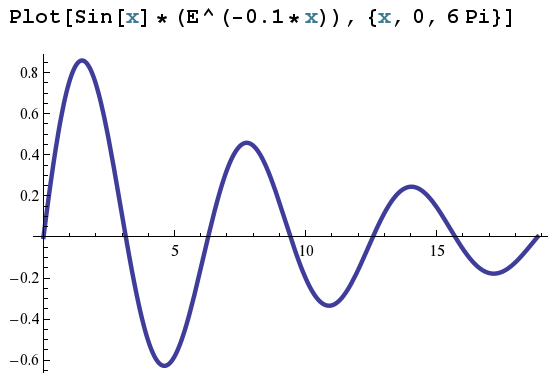
\includegraphics[width=6cm]{Imagenes/Estable.png}
  \end{center}
    \caption{Sistema estable}
  \label{sis_estable}
\end{figure}

\textbf{Sistemas marginalmente estables:} Son aquellos para los cuales una entrada acotada produce una salida acotada por un valor constante $k$, donde $k < \infty$ (véase Figura~\ref{sis_criestable}).

\begin{figure}[ht]
  \begin{center}
    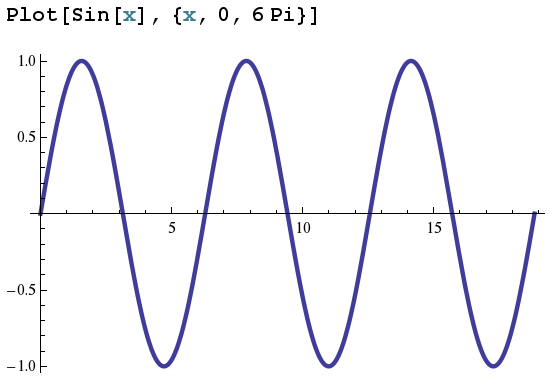
\includegraphics[width=6cm]{Imagenes/Critica.png}
  \end{center}
    \caption{Sistema marginalmente estable}
  \label{sis_criestable}
\end{figure}

\textbf{Sistemas inestables:} Son aquellos para los cuales una entrada acotada produce una salida no acotada (véase Figura~\ref{sis_inestable}).

\begin{figure}[ht]
  \begin{center}
    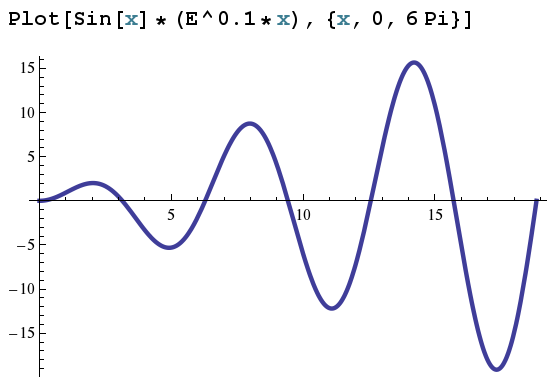
\includegraphics[width=5cm]{Imagenes/Inestable.png}
  \end{center}
    \caption{Sistema inestable}
  \label{sis_inestable}
\end{figure}
\newpage

\item {\bf Sistemas mediante ecuaciones recursivas \par} \cite{edumat}
Los sistemas dinámicos constituyen una rama de la matemática que estudia los procesos en movimiento. Es posible simular cualquiera de estos procesos mediante una función calculada sucesivamente mediante iteraciones. La iteración permite, a partir de un valor $x_i$ en un instante de tiempo $t$, calcular otro valor $x_{i+1}$ en el tiempo $t+\Delta t$ mediante reglas en las que el tiempo no interviene explícitamente. La expresión general de la ecuación iterada sería (Ecuación~\ref{ecua_recursiva}):

\begin{equation}
	x_{i + 1} = f ( x_i )
	\label{ecua_recursiva}
\end{equation}

Utilizando las funciones elementales que incluye una calculadora científica se pueden estudiar sistemas dinámicos simples. Por ejemplo, a partir de un valor inicial $x_0$, pulsando sucesivamente la tecla de la raíz cuadrada estaremos simulando el sistema dinámico: $x_{i +1} = \sqrt{x_i}$, que tiende al valor $1$ (llamado atractor del sistema).

La evolución del sistema depende a veces del punto inicial $x_0$, dando origen a puntos fijos (no cambian al iterarlos), comportamientos periódicos, caóticos, etc. Una órbita (conjunto de puntos iterados) es estable si al iniciar una iteración con un valor “muy próximo” al tomado para la iteración anterior, el resultado no sufre de alguna alteración importante en sus valores.

\item {\bf La ecuación de Malthus \par}
Queremos estudiar la evolución de una población de una determinada especie. Llamamos $x_i$ al número de individuos de la población en el instante temporal $i$. Si suponemos que por cada individuo existente en el período $i$ habrá, por término medio, $k$ individuos en el período $i+1$, se tendrá (Ecuación~\ref{ecua_malthus}):

\begin{equation}
	x_{i+1} = k x_i
	\label{ecua_malthus}
\end{equation}

Esta es la llamada ecuación de Malthus, propuesta por un economista y pensador del siglo XIX para estimar la evolución de la población humana. Si $k>1$ , es decir, si existe algún crecimiento vegetativo de la población, los valores de $x_k$ crecen en progresión geométrica y se disparan de forma exponencial, razón por la cual esta ecuación desató una fuerte polémica entre los contemporáneos de Malthus, suponiendo el primer aldabonazo en la conciencia colectiva de la humanidad sobre el problema de la superpoblación del planeta.

En la representación gráfica se incluye junto a la serie temporal, un gráfico de “telaraña” que representa puntos del tipo $(x_i , x_{i+1}), (x_{i+1},x_{i+1}), (x_{i+1},x_{i+2})$, etc. Estos puntos pertenecen alternativamente a la función $ y=f(x)$ y a la recta $y=x$.

\item {\bf La parabola de May\par}
En 1976 el biólogo Robert May formuló otra ecuación para estudiar el crecimiento de una población de insectos en un ecosistema cerrado, que difería de la de Malthus. May tuvo en cuenta los efectos de saturación del ecosistema, que causan que cuando la población se acerca al máximo posible que el medio ambiente puede sustentar, entonces el parámetro $k$ debe disminuir, lo que equivale a considerar este parámetro función del número de individuos.

Con ello se llega a una ecuación dela forma $x_{i+1} = k(x_i) x_i$ . Podemos tomar como unidad de medida el máximo posible de la población, de manera que $x_i$ expresa la fracción de población existente en el período $i$ con respecto al nivel máximo de población.

May formuló la hipótesis de que $k(x_i)$ debería crecer linealmente cuando $x_i$ creciera, hasta hacerse nulo cuando $x_i$ tomara el valor unidad, es decir, que $k(x_i)$ fuera de la forma $\alpha(1-x_i)$, llegándose así a la ecuación de la parábola logística de May (Ecuación~\ref{ecua_may}):

\begin{equation}
	x_{i+1} = \alpha (1-x_i ) x_i
	\label{ecua_may}
\end{equation}

Se observa que para valores pequeños de $x_i$ se tiene $1-x \approx 1$, con lo que la ecuación resultante es $x_{i+1} = \alpha x_i$ equivalente a la ecuación de Malthus con parámetro $\alpha$. Este parámetro, indica el índice de vitalidad de la población y varía entre cero y cuatro.

\newpage

\item {\bf La dinámica de la parábola logística\par} \cite{carlosPuente}
La ecuación típicamente empleada para explicar el caos es aquella que define la parábola logística o parábola de May (véase Ecuación~\ref{ecua_may}). Aquí, $x_i$ denota el tamaño (normalizado entre 0 y 1) de una población en la generación $i$, $\alpha$ es un parámetro que varía entre 0 y 4 incluidos, y la expresión dicta lo que ocurre de una generación a la siguiente. \\

\begin{figure}[ht]
	\begin{center}
		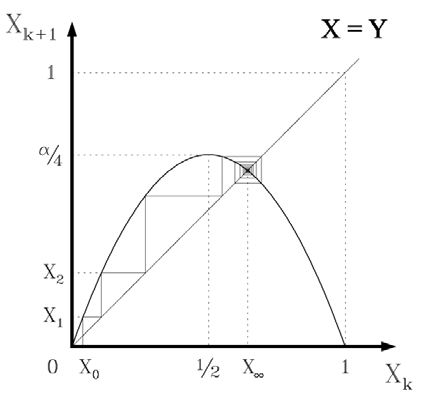
\includegraphics[width=7cm]{Imagenes/logistica_punto_fijo.png}
	\end{center}
	\caption{La parábola logística y la convergencia a un punto fijo}
	\label{logistica_punto_fijo}
\end{figure}

En la Figura~\ref{logistica_punto_fijo} se observa la evolución de una población regida por dicha expresión cuando $\alpha$ es igual a $2,8$. Como se observa, de un valor inicial pequeño $x_0$, y siguiendo sucesivamente las líneas verticales y horizontales hasta la recta $x = y$, se llega, en este caso, a un único punto fijo $x_{\infty}$, que corresponde a la intersección no nula entre la recta y la parábola. De lo anterior se deduce que $x_{\infty}$ depende completamente de $\alpha$. \\

A continuación se repasan los diversos estados que define la simple ecuación cuadrática cuando el pico de la parábola aumenta progresivamente.

\begin{figure}[ht]
	\begin{center}
	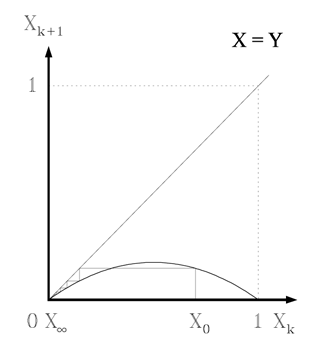
\includegraphics[width=6cm]{Imagenes/logistica_converge_cero.png}
	\end{center}
	\caption{Convergencia al origen}
	\label{logistica_converge_cero}
\end{figure}
\newpage

Cuando la parábola está debajo de la recta, es decir, cuando $\alpha \leq 1$ como en la Figura~\ref{logistica_converge_cero}, $x_{\infty}$ converge a cero, y esto sucede pues la pendiente de la parábola en el origen, al ser menor que la de la recta, atrae cualquier población. Cuando la parábola pasa el umbral uno a uno $x = y$, como en la Figura~\ref{logistica_punto_fijo}, la pendiente de la parábola en el origen es mayor que uno, y entonces la dinámica ya no llega a cero, pues el origen repele. Si $\alpha$ está entre 1 y 3, la reiteración de la ecuación logística converge a la intersección no nula entre la parábola y la recta dada por (Ecuación~\ref{ecua_x_infty}), como en la Figura~\ref{logistica_punto_fijo}.

\begin{equation}
	x_{\infty} = \frac {\alpha - 1} {\alpha}
	\label{ecua_x_infty}
\end{equation} \\

Si $\alpha$ aumenta más allá de $3$, lo que le ocurrió al origen también le sucede a la intersección no nula entre la recta y la parábola, y dicho comportamiento repele. Ahora la dinámica genera oscilaciones estables, primero de dos en dos hasta otro umbral, luego de cuatro en cuatro hasta otro umbral mayor y así sucesivamente, en una cadena de bifurcaciones, tal y como se ilustra en la Figura~\ref{convergencia_ciclos} para valores de $\alpha = 3,2$ (\ref{convergencia_ciclos_a}) y $\alpha = 3,46$ (\ref{convergencia_ciclos_b}).

\begin{figure}[h!]
	\centering
	\subfloat [Caso con $\alpha = 3,2$]{\label{convergencia_ciclos_a} 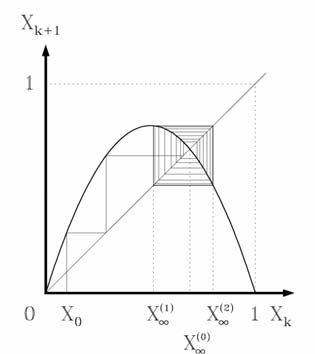
\includegraphics[width=6cm]{Imagenes/convergencia_ciclos_a.png}}
	\hspace{0cm}
	\subfloat [Caso con $\alpha = 3,46$]{\label{convergencia_ciclos_b} 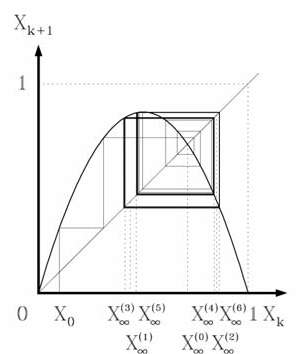
\includegraphics[width=5.6cm]{Imagenes/convergencia_ciclos_b.png}}
	\caption{Convergencia a ciclos repetidos cada 2 y cada 4 generaciones}
	\label{convergencia_ciclos}
\end{figure}
\newpage
Cuando $\alpha$ excede $\alpha_{\infty}$ (el cual se puede calcular en $\alpha_{\infty} \approx 3.5699 $), se encuentran a veces oscilaciones estables como en la Figura~\ref{convergencia_ciclos2}, para valores de $\alpha$ iguales a $3,74$ (\ref{convergencia_ciclos2_a}) y $3,83$ (\ref{convergencia_ciclos2_b}), pero más comúnmente comportamientos infinitos no repetitivos y sujetos a variaciones extremas a condiciones iniciales como en la Figura~\ref{convergencia_atrayentes}, para valores de $\alpha$ de $3,6$ (\ref{convergencia_atrayentes_a}) y $4$ (\ref{convergencia_atrayentes_b}). 

\begin{figure}[h!]
	\centering
	\subfloat [Caso con $\alpha = 3,74$]{\label{convergencia_ciclos2_a} 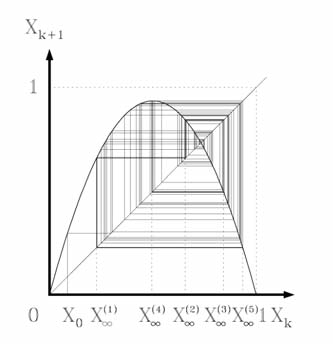
\includegraphics[width=6cm]{Imagenes/convergencia_ciclos2_a.png}}
	\hspace{0cm}
	\subfloat [Caso con $\alpha = 3,83$]{\label{convergencia_ciclos2_b} 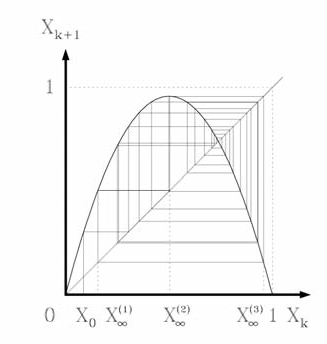
\includegraphics[width=6cm]{Imagenes/convergencia_ciclos2_b.png}}
	\caption{Convergencia a ciclos repetidos cada 5 y cada 3 generaciones}
	\label{convergencia_ciclos2}
\end{figure}

\begin{figure}[h!]
	\centering
	\subfloat [Caso con $\alpha = 3,6$]{\label{convergencia_atrayentes_a} 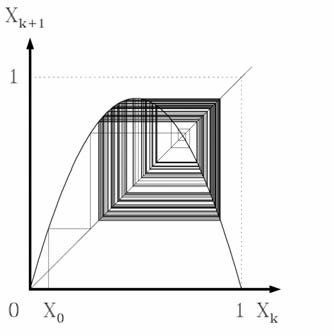
\includegraphics[width=6cm]{Imagenes/convergencia_atrayentes_a.png}}
	\hspace{0cm}
	\subfloat [Caso con $\alpha = 4$]{\label{convergencia_atrayentes_b} 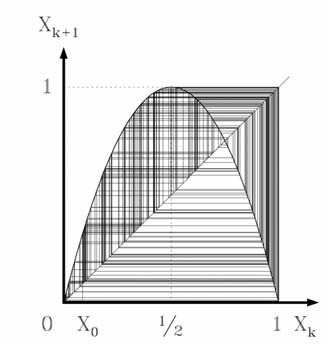
\includegraphics[width=6cm]{Imagenes/convergencia_atrayentes_b.png}}
	\caption{Convergencia a atractores extraños no repetitivos}
	\label{convergencia_atrayentes}
\end{figure} 
\newpage
Resulta ser cierto que existen valores de $\alpha$ mayores que $\alpha_{\infty}$ para los cuales la población se repite exactamente cada $n$ generaciones para cualquier número $n$ que no es una potencia de $2$. Pero, entretejida en esta increíble repetitividad arbitraria, existen muchísimos valores del parámetro $\alpha$ para los cuales la población no se repite, sino que vaga para siempre en un atractor extraño infinito conformado por puntos que no se tocan y que definen el bien denominado comportamiento ``caótico''.

\item {\bf El Árbol de Feigenbaum \par}
La Figura~\ref{bifur_logistica} resume el increíble comportamiento de la sencilla parábola logística. Éste es el famoso diagrama de las bifurcaciones, o el árbol de Feigenbaum.
 
\begin{figure}[ht]
	\begin{center}
		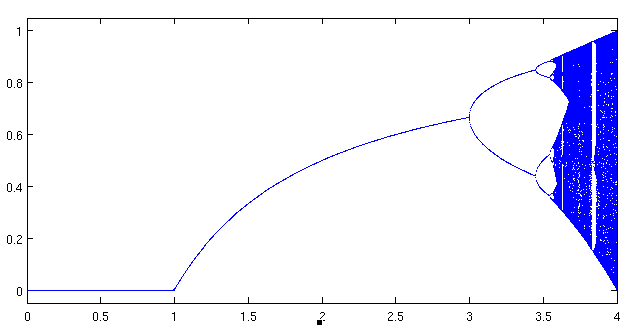
\includegraphics[width=12cm]{Imagenes/bifur_logistica.png}
	\end{center}
	\caption{El árbol de bifurcaciones para la parábola logística}
	\label{bifur_logistica}
\end{figure}

Tal y como puede apreciarse mejor en la Figura~\ref{bifur_logistica_espacios}, en el árbol caótico de Feigenbaum contiene oscilaciones que terminan abarcando, en una infinidad de franjas blancas y en las potencias de 2 previas, todos los números.

\begin{figure}[ht]
	\begin{center}
		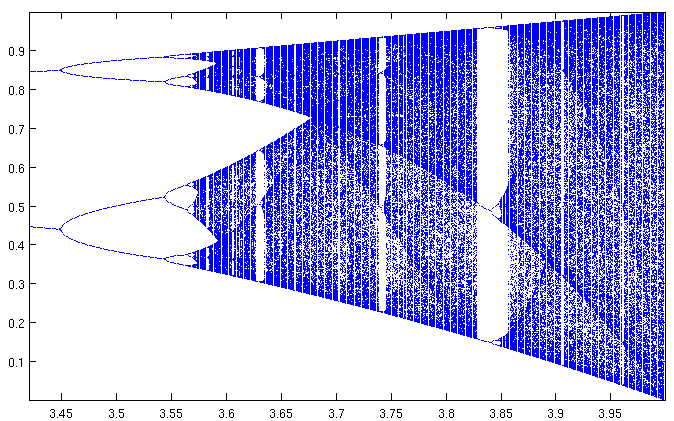
\includegraphics[width=12cm]{Imagenes/bifur_logistica_espacios.png}
	\end{center}
	\caption{La cola del diagrama de bifurcaciones para la parábola logística}
	\label{bifur_logistica_espacios}
\end{figure}

Mitchell Feigenbaum también encontró que las bifurcaciones sucesivas exhiben un orden universal, tanto en las duraciones de las mismas entre umbral y umbral, $\Delta_n$, y las distancias de una rama a la más cercana a partir de una línea que cruza todas las bifurcaciones, $d_n$.

Específicamente, Feigenbaum mostró que el cociente sucesivo de dichas cantidades converge a los números universales $F_1$ y $F_2$ (Ecuaciones \ref{feigenbaum1} y \ref{feigenbaum2}):

\begin{equation}
	\frac {d_n} {d_{n+1}} \rightarrow F_1 \approx -2,503
	\label{feigenbaum1}
\end{equation}

\begin{equation}
	\frac {\Delta_n} {\Delta_{n+1}} \rightarrow F_2 \approx 4,669
	\label{feigenbaum2}
\end{equation}

Y esto resulta ser cierto no sólo para la parábola logística al principio del diagrama de las bifurcaciones, sino para cualquiera de los infinitos brotes dentro del árbol.

Aunque Feigenbaum no descubrió el diagrama de las bifurcaciones, fue él quien encontró que existía un orden en el camino del orden al caos mediante una cadena de bifurcaciones arbitraria, pues las constantes universales de Feigenbaum $F_1$ y $F_2$ no sólo son válidas para la ecuación logística sino que lo son también para una infinidad de ecuaciones que tienen un pico, tal y como se ilustra en la Figura~\ref{bifur_dos_ecuaciones} para dos ecuaciones sencillas.

\begin{figure}[h!]
	\centering
	\subfloat [$x_{k+1} = \alpha x_k (1 - x_k^3)$]{\label{bifur_dos_ecuaciones_a} 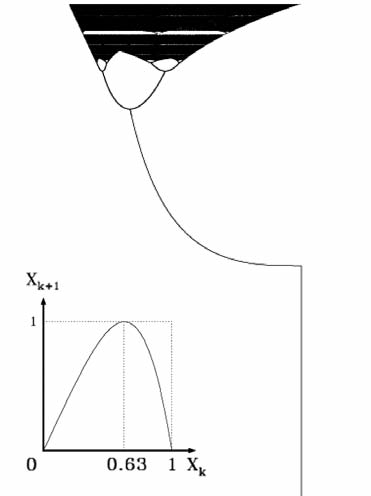
\includegraphics[width=7cm]{Imagenes/bifur_dos_ecuaciones_a.png}}
	\hspace{0cm}
	\subfloat [$x_{k+1} = \alpha x_k (1 - x_k)^3$]{\label{bifur_dos_ecuaciones_b} 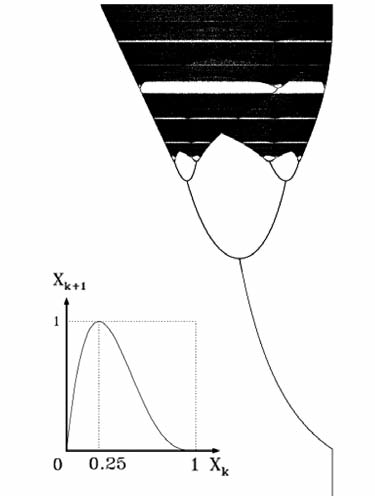
\includegraphics[width=7cm]{Imagenes/bifur_dos_ecuaciones_b.png}}
	\caption{Bifurcaciones para dos ecuaciones no lineales sencillas}
	\label{bifur_dos_ecuaciones}
\end{figure}

\newpage
\item {\bf El efecto mariposa \par} \cite{edumat}
Cuenta Ian Stewart en su libro \textit{¿Juega Dios a los dados?} \cite{Stewart}, que el meteorólogo Edward Lorenz, con el objeto de predecir el tiempo, estaba iterando un complejo sistema dinámico con su ordenador para ver cómo se comportaba en un período de tiempo más grande. En vez de esperar durante varias horas, paró su ordenador y anotó los valores de la órbita en un instante intermedio de lo que ya había realizado, con la intención de volver a ponerlo a funcionar luego de una taza de té.

Un tiempo después puso de nuevo a funcionar su ordenador, para seguir calculando la órbita, con los datos iniciales que había tomado en aquel instante intermedio. Lo que él esperaba que ocurriese es lo siguiente: la máquina repetiría la segunda mitad de la ejecución original, y luego seguiría a partir de allí. La repetición servía como una comprobación útil, pero ahorrándose la primera mitad.

Cuando Lorenz regresó de tomar su taza de té, encontró que la nueva ejecución no había repetido la segunda mitad de la original. Empezaba de la misma manera pero lentamente las dos ejecuciones divergían, hasta que al final no guardaban ningún parecido la una a la otra.

% James Gleik, un escritor científico que se entrevistó con Lorenz, cuenta en su libro \textit{Caos} lo que sucedió a continuación:

De repente comprendió la verdad. No había habido un mal funcionamiento. El problema residía en los números que había introducido. En la memoria del ordenador se almacenaban seis cifras decimales: 0,506127. En la impresión para ahorrar espacio, sólo aparecían tres: 0,506. Lorenz había introducido los números redondeados suponiendo que la diferencia, del orden de las milésimas, no tendría consecuencias.

A consecuencia de esto, Lorenz ideó su famosa frase “efecto mariposa”, para explicar lo sucedido: El movimiento de una simple ala de una mariposa en China, hoy produce un diminuto cambio en el estado de la atmósfera. Después de un cierto período de tiempo, el comportamiento de la atmósfera diverge del que debería haber tenido. Así que, en el período de un mes, un tornado que habría devastado la costa de América no se forma. O quizás uno que no se iba a formar, se produce.

En un sistema dinámico la sensibilidad a las condiciones iniciales se miden mediante un exponente, llamado exponente de Liapunov que determina la tasa de divergencia exponencial de las órbitas adyacentes infinitamente próximas:

Si $x_{i+1} = f(x_i)$ y se tiene que $x_0$ y $x_0 + \varepsilon$ son dos puntos próximos, después de $n$ iteraciones se tiene (Ecuación \ref{ecua_error_exp}):

\begin{equation}
	\lvert f_n (x_0 +\varepsilon ) - f_n (x_0) \rvert = \varepsilon  e^{n \lambda ( x_0 )}
	\label{ecua_error_exp}
\end{equation}

Para determinar el exponente de Liapunov $ \lambda(x_0)$ que determina la divergencia, mediante logaritmos se obtiene una aproximación para $n$ iteraciones (Ecuación \ref{ecua_error_ln}):

\begin{equation}
	\lambda ( x_0 ) = \frac{1}{n} \ln  \left | \frac {f_n ( x_0 + \varepsilon) - f_n ( x_0 )} {\varepsilon}  \right |
	\label{ecua_error_ln}
\end{equation}

El auténtico valor se obtiene tomando límites cuando $n$ tiende a infinito y $\varepsilon$ tiende a cero.

% \item {\bf Teoría del caos \par}
\subsubsection{Teoría del caos}
Es el campo de estudio de las matemáticas, física, economía, filosofía y otras áreas del conocimiento que estudia el comportamiento de los sistemas dinámicos que son altamente sensibles a leves variaciones en sus condiciones iniciales. Esta sensibilidad se puede notar cuando partiendo de dos estados iniciales muy similares en un sistema caótico puede desarrollarse de maneras radicalmente diferentes. \cite{Angel08}

El término caos no puede confundirse con ausencia de orden, ya que su significado matemático está relacionado con la falta de certidumbre que produce al intentar predecir los futuros estados de un sistema. Tampoco se debe asociar el concepto de caos con el de aleatoriedad, ya que el hecho de no poder determinar de manera precisa el comportamiento de un sistema, no obliga a este a ser no-determinista.

\item {\bf Sistemas caóticos \par}
Un sistema es caótico si la relación entre las entradas y las salidas del mismo presenta un comportamiento caótico. En otras palabras, un sistema es caótico si cumple al menos una de las siguientes características:
\begin{itemize}
 \item Pequeños cambios en las condiciones iniciales del sistema desembocan en grandes cambios en la salida del mismo. Esto también se puede ver como que pequeños \emph{errores} en la medición de las entradas de un sistema caótico, hacen que la predicción de su salida sea totalmente errónea.
 \item Siendo un sistema dependiente de mucha variables, cualquier simplificación aplicada al sistema que incluya la omisión de variables, desemboca en un erróneo modelamiento del sistema. En otras palabras, se consideran sistemas caóticos a aquellos que no son modelables mediante la mecánica clásica debido a que el número de variables necesarias para su correcta modelación es inmanejable.
\end{itemize}

\newpage

% \item {\bf Atractores extraños\par} \cite{caos_atractores}
\subsubsection{Atractores extraños} \cite{caos_atractores}
Un atractor se pueden definir como el conjunto al que todas las trayectorias vecinas convergen, o mas estrictamente como el conjunto cerrado que cumple con las siguientes propiedades:

\begin{itemize}
	\item Invariantes frente a la dinámica del sistema: cualquier trayectoria que comienza en el atractor permanece en él indefinidamente.
	\item Atrae a un conjunto abierto de condiciones iniciales cercanos a él. Al conjunto más grande se llama cuenca de atracción.
	\item Es un conjunto mínimo: ningún subconjunto de él puede satisfacer las propiedades anteriores.
\end{itemize}

En los sistemas no caóticos el atractor suele ser un punto, una circunferencia, una figura geométrica conocida, pero en los sistemas caóticos presenta una forma “extraña”, de ahí que reciba el nombre de “atractor extraño”, con una dimensión fraccionaria o fractal.\cite{bellateoria} El atractor mas conocido es el de Lorenz, el cual se aprecia en la Figura~\ref{lorenz}.

\begin{figure}[h!]
	\centering
	\subfloat [Proyección en 2D del atractor de Lorenz]{\label{lorenz2d} 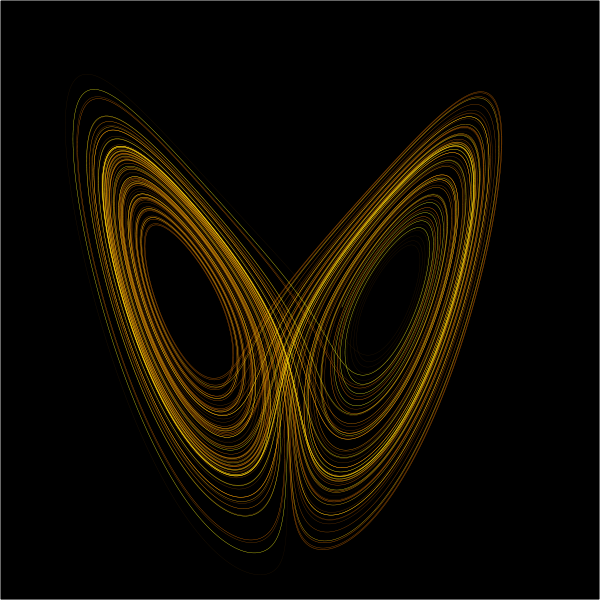
\includegraphics[width=7cm]{Imagenes/lorenz2d.png}}
	\hspace{0cm}
	\subfloat [Atractor de Lorenz en 3D]{\label{lorenz3d} 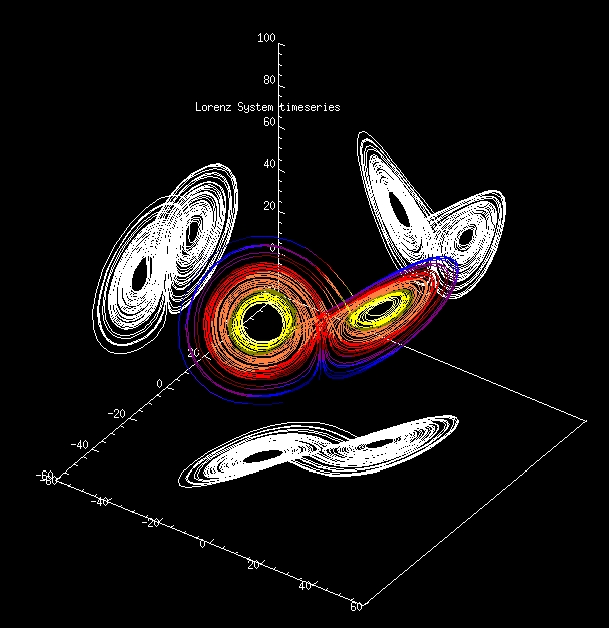
\includegraphics[width=6.8cm]{Imagenes/lorenz3d.jpg}}
	\caption{Diferentes formas del atractor de Lorenz}
	\label{lorenz}
\end{figure}

\newpage
\subsubsection{Fractal}
Los fractales son representaciones gráficas de ciertos conjuntos de datos, los cuales generan repetición de patrones (parciales o totales) a lo largo del dibujo. Esta representación produce  objetos semi-geométricos no euclidianos.

La palabra fractal viene del latín \textit{fractus} que significa fracturado, quebrado. Este nombre se debe a que muchos poseen una estructura que al ser fragmentada se repite en diferentes escalas (auto similar). Muchos se pueden dibujar siguiendo un algoritmo recursivo y otros usando técnicas aleatorias.

Los fractales no son simples abstracciones matemáticas, sino que son representaciones de una realidad tangible en la naturaleza. Se pueden encontrar numerosos ejemplos de fractales: las nubes, el sistema circulatorio, los copos de nieve, etc.

Entre los fractales mas conocidos encontramos (véase Figura~\ref{ejemp_frac}):
% \begin{itemize}
%  \item Curva de Koch
%  \item Conjuntos de Jilia
%  \item Cunjunto de Mandelbrot
% \end{itemize}

\begin{figure}[h!]
\centering
	\subfloat [Generación de Curva de Koch]{\label{koch_gen} 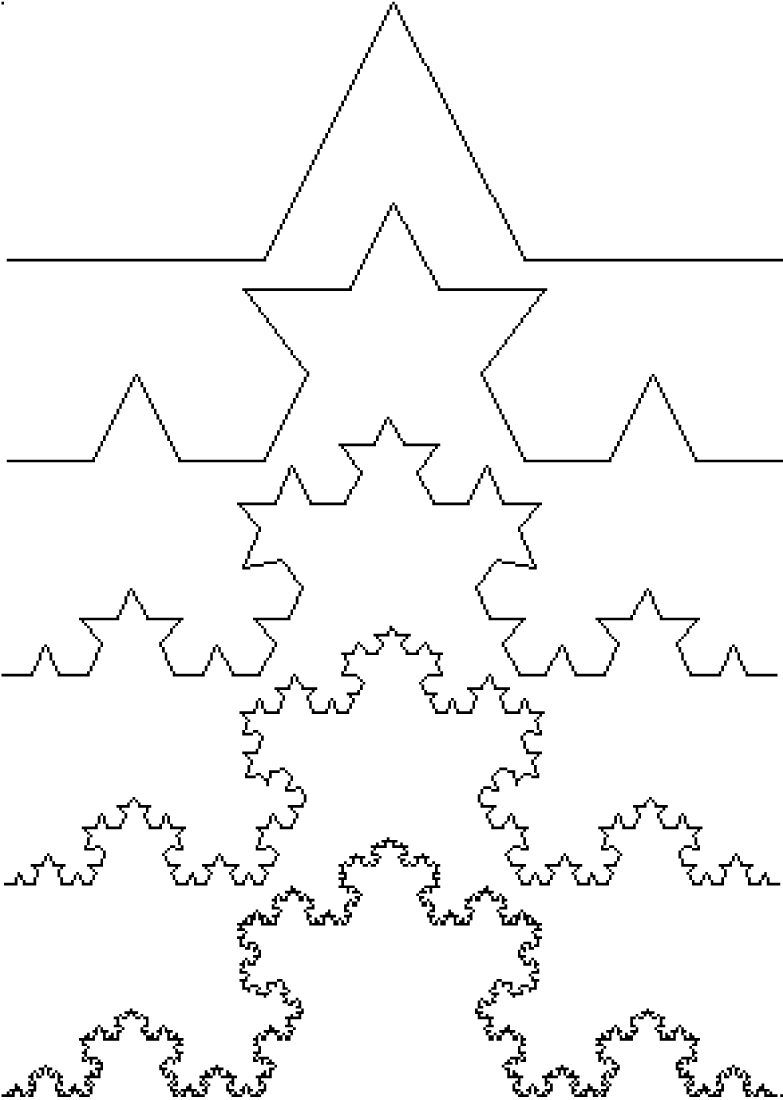
\includegraphics[width=3.2cm]{Imagenes/koch_gen.png}}
	\hspace{0cm}
	\subfloat [Conjunto de Julia]{\label{julia} 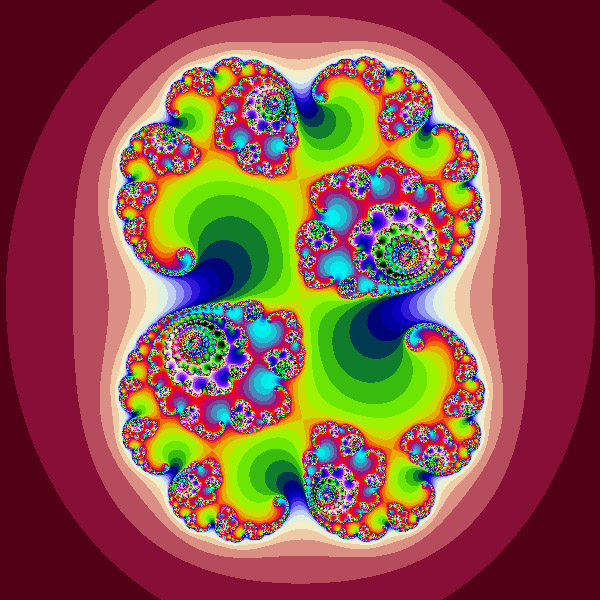
\includegraphics[width=4cm]{Imagenes/julia.jpg}}
	\hspace{0cm}
	\subfloat [Conjunto de Mandelbrot]{\label{mandelbrot} 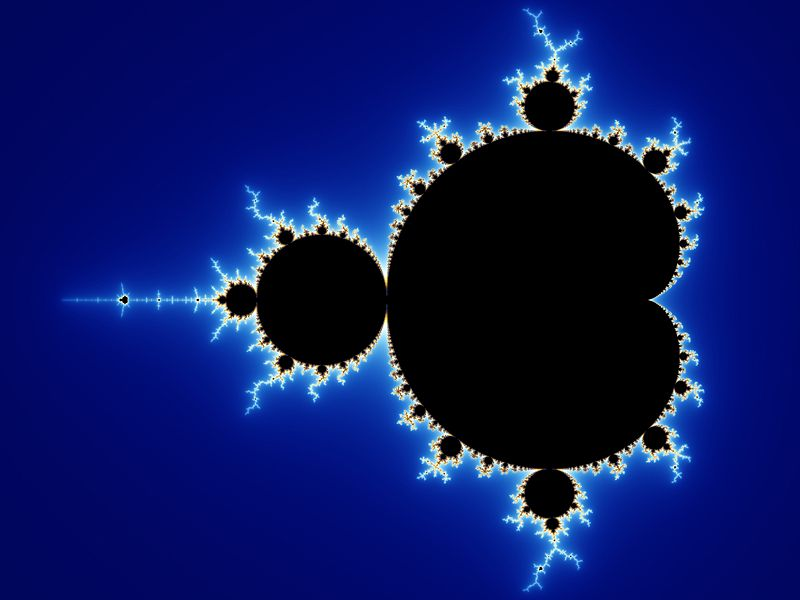
\includegraphics[width=7.5cm]{Imagenes/mandelbrot.jpg}}
\caption{Ejemplos de fractales}
\label{ejemp_frac}
\end{figure}

\end{itemize}
\clearpage

\subsubsection{Aplicaciones de la teoría del caos y de los fractales}
\begin{itemize}
\item {\bf El Caos en la naturaleza \par}

Las formas fractales se observan en todo lo que es natural, y a todas las escalas.\cite{multimania}


\begin{figure}[ht]
	\begin{center}
		
\includegraphics[width=7cm]{Imagenes/helecho.jpg}
	\end{center}
	\caption{Helecho artificial}
	\label{helecho}
\end{figure}

La figura \ref{helecho} es de un fractal: parece un helecho, pero en realidad es un gráfico de puntos esparcidos caóticamente por la reiteración de una fórmula no lineal.
Parece que el mundo de los fractales numéricos y el mundo fractal material forman parte de un mismo fractal, puesto que contienen formas casi idénticas. El mundo entero es un fractal que se autoasemeja a diferentes escalas. Sin embargo los fractales matemáticos son mucho más simplificados. A menudo la naturaleza ofrece un desafío a la descripción: las autosemejanzas de sus formas están combinadas con una inagotable novedad, que no puede ser descrita ni siquiera por algoritmos no lineales. \\

{\bf La autoorganización de colonias de hormigas: }Su comportamiento global sorprende: si contamos el número de individuos activos, a lo largo del tiempo, comprobaremos que el número fluctúa con una periodicidad de unos 25 minutos. Cada cierto tiempo ningún elemento está activo. Ese ciclo de actividad podría ser sólo un reflejo de sincronización, sin embargo la actividad individual es totalmente aperiódica, caótica, sin ningún tipo de regularidad intrínseca. 
Al aumentar el número de individuos aparece un comportamiento colectivo hasta que, para cierta densidad de hormigas, comienzan a aparecer oscilaciones regulares. Si artificialmente cambiamos la densidad de las hormigas la colonia redefine sus fronteras, para volver a la densidad óptima para mantenerlas autoorganizadas. En esa densidad crítica el sistema se comporta como un todo, a medio camino entre el orden y el desorden. \\

{\bf La macroevolución: } El proceso evolutivo se puede representar en forma de árbol, cuya estructura dendriforme es fractal. Las regularidades que aparecen entre grupos taxonómicos revelan la existencia de leyes invariantes a cualquier escala taxonómica, propiedad típica de los fractales.
El 99,99\% de las formas vivientes que han aparecido sobre la Tierra se han extinguido. 
Si la adaptación confiere ventaja a la especie, cabe presumir que los grupos más persistentes serán los menos propensos a desaparecer. Pero el estudio de los patrones de extinción nos dice que la probabilidad de extinción de un grupo cualquiera se muestra constante a lo largo del tiempo y no depende de cuánto llevara existiendo en el planeta.
En su teoría, Van Valen considera que cada especie intenta mejorar su posición dentro del ecosistema: además de interaccionar con el medio físico también interacciona con el ambiente biótico. Un cambio en la situación de una especie induce a cambios en las demás, cuya alteración influirá, a su vez, en la primera, y así en idas y venidas sin fin. Así el sistema evoluciona hacia un punto crítico donde se aprecia que ciertas partes del sistema permanecen inalteradas durante largo tiempo, mientras que otras se modifican con rapidez. 
La especie cambia sólo para persistir: la selección natural no mejora la adaptación de la especie: sólo la mantiene. Las especies incapaces de cambiar se extinguen.

\item {\bf El caos aplicado a la inteligencia artificial \par}

Una de las aplicaciones más directas y que actualmente se realizan más estudios es la aplicación en el campo de la inteligencia artificial. El ejemplo de las hormigas se puede comparar con una red neural fluida en la inteligencia artificial. La fluidez en un sistema caótico se manifiesta cuando las conexiones entre elementos cambian con el tiempo como consecuencia del movimiento al azar o por otras causas. Un elemento (una hormiga, una neurona) que está inmóvil puede volver a la actividad ya sea por interacción o de forma espontánea, siendo las actividades espontáneas totalmente caóticas. Así, a baja densidad de elementos, las fluctuaciones serían muy irregulares porque habría poca interacción y los elementos no pr opagan bien sus cambios. A grandes densidades las fluctuaciones del sistema se tornan periódicas: la activación de un elemento se propaga en forma de onda. Pero entre ambos extremos (irregularidad y periodicidad) existe una densidad crítica, un punto de bifurcación, en el cual la información transmitida se hace máxima. La computación (la capacidad de un sistema complejo para captar y procesar información) a menudo aparece en la naturaleza cuando un sistema caótico llega a un punto crítico. Para procesar información se necesita un cierto grado de orden interno, que permita almacenar temporalmente cierta información. Pero la información ha de ser manipulable, por eso el desorden es necesario, para permitir la fluidez del sistema caótico.

La idea de introducir la aleatoriedad en los sistemas de IA también se puede observar de otro modo. En la teoría del caos la aleatoriedad es simplemente algo que no comprendemos por qué pasa, es una pequeña porción del fractal que forma el mundo. Teniendo en cuenta las propiedades de los fractales (autosemejanza a diferentes escalas) es posible coger esa porción de fractal y, estudiándola desde una escala adecuada (es decir, descubriendo un punto crítico), descubrir el contexto de la información dentro del sistema fractal.

\item {\bf Compresión de imágenes \par}

Una de las aplicaciones más útiles de los fractales y de la geometría fractal está en la compresión de imágenes. Es también una de las ideas con más controversia. El concepto básico detrás de la compresión fractal de imágenes es tomar una imagen y expresarla como un Sistema de Funciones Iteradas (SFI). Un SFI es el conjunto de funciones que describen partes de un fractal que, una vez juntas, recrean dicho fractal en su totalidad. Si un fractal puede ser descrito por un número pequeño de funciones, el SFI es una descripción bastante compacta del fractal. La imagen puede ser rápidamente desplegada y a cualquier grado de magnificación con infinitos niveles de detalle fractal. El mayor problema detrás de esta idea es encontrar el SFI que describa la imagen. 

\item {\bf Efectos visuales \par}

Una de las más triviales aplicaciones de los fractales son sus efectos visuales. No solamente engañan la vista, sino que también de algún modo confunden a la mente. Los fractales han estado siendo usados comercialmente en la industria cinematográfica, en películas como Star Wars y Star Trek. Las imágenes fractales son usadas como una alternativa para producir paisajes de gran imaginación. 

\item {\bf Música fractal \par}

Otra aplicación de los fractales aparentemente irrelevante es la música fractal. Ciertas músicas, incluyendo las de Bach y las de Mozart, pueden ser reducidas y todavía retener la esencia del compositor. Están siendo desarrolladas muchas nuevas aplicaciones software para el desarrollo de música fractal.
\end{itemize}

\newpage

\subsection{Conceptos pedagógicos} %%% Posibilidad de buscar mas o de expandir
\begin{itemize}

\item \textbf{Objeto virtual de aprendizaje:} “Cualquier entidad digital que puede ser usada, reutilizada o referenciada durante un proceso de aprendizaje apoyado por la tecnología” \cite{IEEE2006} o también según el ministerio de educación nacional, “un objeto virtual es un mediador pedagógico que ha sido diseñado intencionalmente para un propósito de aprendizaje y que sirve a los actores de las diversas modalidades educativas” \cite{Roldan05}. 
En tal sentido, dicho objeto debe diseñarse a partir de criterios como: 
\begin{itemize}
\item Atemporalidad: Para que no pierda vigencia en el tiempo y en los contextos utilizados. 
\item Didáctica: El objeto tácitamente responde a qué, para qué, con qué y quién aprende. 
\item Usabilidad: Que facilite el uso intuitivo del usuario interesado. 
\item Interacción: Que motive al usuario a promulgar inquietudes y retornar respuestas o experiencias sustantivas de aprendizaje. 
\item Accesibilidad: Garantizada para el usuario según los intereses que le asisten. 
\end{itemize}
\end{itemize}
\clearpage
\subsection{Conceptos de desarrollo de software}

\begin{itemize}
\item \textbf{PHP :} Acrónimo de "PHP: Hypertext Preprocessor", es un lenguaje open source interpretado de alto nivel, especialmente pensado para desarrollos web y el cual puede ser incrustado en páginas HTML. La mayoría de su sintaxis es similar a C, Java y Perl y es fácil de aprender. La meta de este lenguaje es permitir escribir a los creadores de páginas web, páginas dinámicas de una manera rápida y fácil, aunque se pueda hacer mucho más con PHP. \cite{PHP}

PHP es un lenguaje interpretado de alto nivel embebido en páginas HTML y ejecutado en el servidor. La comunicación entre el cliente y el servidor con PHP se realiza de la siguente manera: un servidor web (que puede ser el Apache, IIS, etc.) recibe una petición y al ver que la extension es “.php” solicita al interprete de PHP (que es otro programa que se ejecuta en el servidor web) que procese el archivo de la petición. El intérprete PHP ejecuta los comandos contenidos en el archivo y eventualmente se comunica con un gestor de base de datos (ejemplos de ellos pueden ser MySql, PostgreSql ,Oracle, Informix, SQL Server, etc.), Después de ejecutar el programa contenido en el archivo envía el resultado al servidor web y finalmente al cliente que la había solicitado.

\item \textbf{Sistema de gestión de contenidos :} Abreviado CMS, en inglés Content Management System, es una herramienta que permite crear una estructura de soporte para la creación y administración de contenidos, principalmente en páginas web.

Consiste en una interfaz que controla una o varias bases de datos donde se aloja el contenido del sitio. El sistema permite manejar de manera independiente el contenido y el diseño. Así, es posible manejar el contenido y darle en cualquier momento un diseño distinto al sitio sin tener que darle formato al contenido nuevamente.

El gestor de contenidos es usado entonces para crear, editar y publicar contenido digital en diversos formatos, generando páginas dinámicas a través de la interacción con el servidor, con el formato predefinido y el contenido extraído de la base de datos del servidor. Esto permite gestionar, bajo un formato estandarizado, la información del servidor, reduciendo el tamaño de las páginas para descarga y reduciendo el coste de gestión de la aplicación web con respecto a una página estática, en la que cada cambio de diseño debe ser realizado en todas las páginas, de la misma forma que cada vez que se agrega contenido tiene que construirse una nueva página.

Entre los gestores de contenido más comúnmente usados se encuentran Drupal, Joomla! y Radiant entre una gran cantidad en varios lenguajes de programación.

\item \textbf{Drupal :} \cite{Drupal} \cite{Drupal2} Es un sistema manejador de contenidos de código abierto que es utilizado por cientos de miles de organizaciones y personas para construir atractivos sitios web ricos en contenido. Es un programa de código abierto, con licencia GNU/GPL, escrito en PHP, desarrollado y mantenido por una activa comunidad de usuarios. Destacado por la calidad de su código y de las páginas generadas con respecto a los estándares web y de usabilidad y consistencia de todo el sistema.

El diseño de Drupal es especialmente idóneo para construir y gestionar comunidades en Internet. No obstante, su flexibilidad y adaptabilidad, así como la gran cantidad de módulos adicionales, hace que sea adecuado para realizar muchos tipos de sitios.

La construcción de un sitio web en Drupal se basa en combinar varios ``bloques de construcción'' con el fin de personalizar la funcionalidad de su sitio web a sus necesidades precisas. Una vez construido, un sitio web en Drupal se puede mantener con formularios en línea, y sin tener que cambiar el código manualmente. 

Drupal es un framework para la gestión y administración de contenido de contenido modular y muy configurable. Además de proporcionar herramientas de creación de sitios para los administradores, ofrece mecanismos para que los programadores y desarrolladores personalicen Drupal mediante extensiones. Casi todo en Drupal se puede personalizar mediante estos módulos, y existen miles de ellos que incorporan más características. La mayoría de los módulos han sido aportados por la comunidad de Drupal y están disponibles para descargar y utilizar en su sitio web.

Drupal es una herramienta que ayuda a construir sitios y aplicaciones web de forma interactiva de una manera agradable y sencilla. Drupal ha sido galardonado por tercera vez consecutiva como el mejor sistema manejador de contenidos de la actualidad por la comunidad. Su escalabilidad y sus bajos costos de licencia y mantenimiento lo convierten en la mejor opción para encarar proyectos de mediana a gran envergadura. Drupal puede ser considerado como:
\begin{itemize}
\item Una aplicación web fuertemente apoyada en base de datos donde toda su información y el contenido de la aplicación es almacenada en esta.
\item Un proyecto de software libre para la gestión de contenidos web.
\item Una plataforma construida por la comunidad. Su estructura permite fácilmente que cualquier persona pueda crear un módulo, un tema o colabore con el desarrollo de la plataforma como tal.
\item Una plataforma de desarrollo web que utiliza el patrón de diseño modelo vista controlador. Permitiendo crear desarrollos personalizados e integrados totalmente a la plataforma.
\end{itemize}

\item \textbf{HTML 5 :} \cite{HTML5} Lenguaje de programación que predomina en la elaboración de páginas web por su sencillez y fácil comprensión. En su quinta versión, se introducen nuevas características y elementos basados en la investigación sobre las prácticas actuales de creación de aplicaciones web, y se ha prestado especial atención a la definición de criterios claros en un esfuerzo por mejorar la interoperabilidad.\\

HTML 5 establece una serie de nuevos elementos y atributos que reflejan el uso típico de los sitios web modernos. Algunos de ellos son técnicamente similares a las etiquetas \textless div\textgreater y \textless span\textgreater, pero tienen un significado semántico, como por ejemplo \textless nav\textgreater (bloque de navegación del sitio web) y \textless footer\textgreater (pie de pagina). Otros elementos proporcionan nuevas funcionalidades a través de una interfaz estandarizada, como los elementos \textless audio\textgreater y \textless video\textgreater.\\

HTML 5 incluye novedades significativas en diversos ámbitos. No sólo se trata de incorporar nuevas etiquetas o eliminar otras, sino que supone mejoras en áreas que hasta ahora quedaban fuera del lenguaje y para las que se necesitaba utilizar otras tecnologías. Algunas de las novedades son:
\begin{itemize}
  \item \textbf{Estructura del cuerpo :} La mayoría de las webs tienen un formato común, formado por elementos como cabecera, pie, navegadores, etc. HTML 5 permite agrupar todas estas partes de una web en nuevas etiquetas que representarán cada una de las partes típicas de una página.
  \item \textbf{Etiquetas para contenido específico :} Hasta ahora se utilizaba una única etiqueta para incorporar diversos tipos de contenido enriquecido, como animaciones Flash o vídeo. Ahora se utilizarán etiquetas específicas para cada tipo de contenido en particular, como audio, vídeo, etc.
  \item \textbf{Canvas :} Es un nuevo componente que permitirá dibujar, por medio de las funciones de un API, en la página todo tipo de formas, que podrán estar animadas y responder a interacción del usuario. Es algo así como las posibilidades que nos ofrece Flash, pero dentro de la especificación del HTML y sin la necesidad de tener instalado ningún plugin.
\item \textbf{Bases de datos locales :} El navegador permitirá el uso de una base de datos local, con la que se podrá trabajar en una página web por medio del cliente y a través de un API. Es algo así como las Cookies, pero pensadas para almacenar grandes cantidades de información, lo que permitirá la creación de aplicaciones web que funcionen sin necesidad de estar conectados a Internet.
\item \textbf{Web Workers :} Son procesos que requieren bastante tiempo de procesamiento por parte del navegador, pero que se podrán realizar en un segundo plano, para que el usuario no tenga que esperar que se terminen para empezar a usar la página. Para ello se dispondrá también de un API para el trabajo con los Web Workers.
\item \textbf{Aplicaciones web Offline :} Existirá otro API para el trabajo con aplicaciones web, que se podrán desarrollar de modo que funcionen también en local y sin estar conectados a Internet.
\item \textbf{Geolocalización :} Las páginas web se podrán localizar geográficamente por medio de un API que permita la geolocalización.
\item \textbf{Fin de las etiquetas de presentación :} Todas las etiquetas que tienen que ver con la presentación del documento, es decir, que modifican estilos de la página, serán eliminadas. La responsabilidad de definir el aspecto de una web correrá a cargo únicamente de CSS.
\end{itemize}

\item \textbf{Sistemas de Lindenmayer :}  Es un tipo de gramática formal que permiten la generación de modelos de plantas a través de su producción, Lindenmayer introdujo un método formal para almacenar un tipo de información que representa el crecimiento de organismos multicelulares, que fue conocido posteriormente como sistemas de Lindenmayer o sistemas-L. El desarrollo de este formalismo estaba enfocado en el modelado de arquitecturas para plantas. Para poder describir los modelos de las plantas en general, desde las algas hasta los árboles grandes, Lindenmayer introdujo una notación en forma de cadenas de caracteres, donde cada elemento del lenguaje es interpretado para formar un grafo que representa finalmente la planta. \\

Mas formalmente un sistema de Lindenmayer está conformado por un alfabeto en el que se encuentran todos los posibles caracteres que pueden ser usados en el sistema, una palabra no vacía llamada axioma y un conjunto de reglas finito de producción, donde cada regla de producción está representada por el alfabeto usado y usando un par palabras que son el antecesor y el sucesor de la regla de producción. \\

Un sistema-L es parecido a las gramáticas de los lenguajes formales, excepto por el hecho de que en los sistemas-L las reglas son aplicadas de manera paralela y además  que no hay distinción entre los símbolos terminales y no terminales. El proceso de aplicación de las reglas es llamado proceso de derivación o de reescritura. Los sistemas-L son básicamente generadores de palabras de un determinado lenguaje especificado en el cual está contenida la información a respecto de una figura geométrica. \\

Un algoritmo llamado de gráficos de tortuga es utilizado para interpretar las palabras generadas por los sistemas-L. Su idea principal consiste en una tortuga que ejecuta ciertos comandos de acuerdo con los caracteres contenidos en las palabras. Su estado está representado por tres atributos donde se representa la ubicación bidimensional y el ángulo en el cual está posicionada. La tortuga interpreta cada palabra como un conjunto de segmentos de recta totalmente conectados, o sea que no interesa la forma de la figura, ésta siempre estará formada por un segmento continuo de recta.\\
\end{itemize}

\subsection{Conclusiones del marco teórico}

Los conceptos teóricos nos dan una idea de la complejidad que tiene la teoría del caos y de la cantidad de conceptos relacionados para lograr una comprensión del tema que permita comprenderla y utilizarla para poder resolver problemas. La teoría del caos sirve para comprender las interconexiones del mundo, ayuda a reconocer las causas de ciertos ``acontecimientos fortuitos'' y a estar mejor preparados para afrontarlos.

Los conceptos pedagógicos ilustran la manera como se puede adoptar la enseñanza a sistemas o ambientes virtuales, ya que por medio de un objeto de aprendizaje se crea una estructura autónoma que contiene un objetivo general, objetivos específicos, una actividad de aprendizaje, un meta-dato (estructura de información externa) y por ende, mecanismos de evaluación y ponderación, el cual puede ser desarrollado con elementos multimedia con el fin de posibilitar su reutilización, interoperabilidad, accesibilidad y duración en el tiempo.

Los conceptos de desarrollo de software muestran lo útil de implementar sistemas de gestión de contenido como Drupal. Son una excelente solución para lograr una aplicación rápida y completa. Crear un manejador de contenido desde cero requiere de un gran trabajo y solo es útil cuando los requerimientos son pocos o en entornos muy pequeños, mas sin embargo utilizar uno ya construido nos brinda funcionalidades que son comunes en la mayoría de desarrollos web, y que se encuentran de una forma mas completa, además de que sistemas como los actuales son muy configurables y adaptables llenando las expectativas del desarrollador y del usuario final.

\clearpage
\begin{center}
 \section{Estado del Arte}
\end{center}

Un objeto virtual de aprendizaje enfocado en la enseñanza de la teoría del caos no existe actualmente. Se hará referencia entonces a sistemas de gestión utilizados para la construcción de entornos virtuales de aprendizaje, aplicaciones que muestran de manera didáctica conceptos de la teoría del caos como lo es la visualización de fractales y una revisión a otros objetos virtuales de aprendizaje de otros temas.

\subsection{Sistemas de Gestión de Aprendizaje}

Un entorno virtual de aprendizaje se define como una plataforma tecnológica que trata de reproducir las condiciones y recursos educativos de una clase presencial y proporciona a profesores y estudiantes las facilidades para la comunicación y la interacción; venciendo de esta manera la necesidad de los actores implicados en el proceso de enseñanza-aprendizaje, y de coincidir temporal y geográficamente. \cite{Dorado06}

Para que los objetos de aprendizaje puedan cumplir con los preceptos de reusabilidad, interoperabilidad, mantenibilidad e intercambiabilidad entre diferentes sistemas de gestión o entornos de aprendizaje, estos deben ser desarrollados siguiendo los actuales estándares de enseñanza virtual\cite{Fernandez2006}. Estos estándares son recomendaciones técnicas y metodológicas desarrolladas al interior de organizaciones dedicadas al impulso y consolidación de la enseñanza virtual, las cuales posibilitan la construcción de objetos de aprendizaje que cumplan los preceptos mencionados. Las principales organizaciones en desarrollo de estándares de enseñanza virtual son IEEE\cite{IEEE2006}, ADL/SCORM\cite{SCORM2006}, IMS\cite{IMS2006}.

Un completo sistema de gestión del aprendizaje debe entonces contener los siguientes tipos de herramientas:

\begin{itemize}
\item Herramientas de comunicación: aquellas que permiten a estudiantes y profesores establecer comunicación. Refiriéndonos concretamente a foros, chat o correo electrónico.
\item Herramientas de gestión de usuarios y cursos: Aquellas que permiten a los encargados de la operación del entorno virtual de aprendizaje crear, modificar, eliminar y administrar usuarios y cursos.
\item Herramientas de almacenamiento de archivos: Soportan el proceso de subir, almacenar y descargar diversa documentación necesaria para la orientación de los cursos
\end{itemize}

\subsubsection{Moodle}Es un sistema web para administración de cursos y enseñanza virtual el cual promueve una pedagogía constructivista social. Su arquitectura y herramientas son apropiadas para clases en línea, así como también para complementar el aprendizaje presencial. Tiene una interfaz de navegador de tecnología sencilla, ligera, y compatible.

Contiene varios módulos como lo son tareas, consultas, foros, diarios, cuestionarios, recursos, encuestas, wiki, lo que lo hacen una herramienta con variadas utilidades, mas sin embargo algunas actividades pueden ser un poco mecánicas, dependiendo mucho del diseño instruccional. Por estar basado en tecnología PHP, la configuración de un servidor con muchos usuarios debe ser cuidadosa para obtener el mejor desempeño. Falta mejorar su interfaz para permitir una administración más sencilla. Hay desventajas asociadas a la seguridad, dependiendo en dónde se esté alojando la instalación de Moodle y cuáles sean las políticas de seguridad y la infraestructura tecnológica con la cual se cuente durante la instalación.
Existen también desventajas relacionadas con el soporte técnico. Al ser una plataforma de tecnología abierta y por lo tanto gratuita, no se incluyen servicios gratuitos de soporte por lo que los costos de consultoría y soporte técnico están sujetos a firmas y entidades externas.

\subsubsection{Claroline} \cite{CLAROLINE} \cite{Sampedro} Es un sistema de administración del aprendizaje. Está diseñado para ayudar a profesores e instructores a crear contenidos educacionales y supervisar las actividades de aprendizaje en la web. Permite tanto a estudiantes como a profesores organizar el proceso de aprendizaje, comunicarse entre ellos, auto-evaluarse y manejar un calendario de actividades.

Claroline permite la estructuración de cursos, colocación de material y administración de actividades. Da libertad a los profesores para estructurar y colocar su material de estudio. El proceso de aprendizaje individual como está contemplado en esta herramienta utiliza lecturas y/o documentos en formatos diferentes.

Claroline ha sido desarrollado principalmente para apoyar un buen proceso de enseñanza-aprendizaje, no para substituirlo. Busca ser útil, guiado por los requisitos de los usuarios, abierto para permitir integrar servicios existentes y nuevas herramientas, y adaptable a escenarios concretos para sus cursos. Debido a que Claroline es un software de código abierto y modular, permite a un administrador agregar y modificar herramientas, cambiar la disposición, adaptar bases de datos, etc. Claroline permite personalizar la apariencia del sitio, pero no permite adaptar funcionalidades o agregar nuevos módulos de una forma efectiva o útil.

\subsection{Visualización de fractales}
\subsubsection{XaoS}
Es un programa interactivo de visualización de fractales. Permite al usuario hacer acercamientos a diferentes fractales en tiempo real. XaoS se encuentra bajo la licencia GPL. El programa es multiplataforma, lo que le permite ser ejecutado en variedad de sistemas operativos como GNU/Linux, Windows, Mac OS X, BeOS y otros.
XaoS puede mostrar el conjunto de Mandelbrot ( elevado a la 2, 3, 4, 5 y 6), el octo fractal, tres tipos de fractales de Barnsley entre variedad de otros conjuntos de fractales, además permite entrar fórmulas personalizadas para dibujar fractales por parte del usuario.

Es entonces un visualizador y explorador de diferentes grupos de fractales, que incluye tutoriales para la enseñanza de las características principales de los fractales. Y otras herramientas interesantes como piloto automático, cambio de colores, grabación de vídeo e imágenes, filtros, etc. 
\subsubsection{Fraqtive}
Fraqtive es un generador multiplataforma de fractales de la familia Mandelbrot de código abierto. Usa algoritmos veloces que soportan tecnología SSE2 y procesadores multinúcleo. Genera imagenes antialiasing y escenas en tres dimensaiones usando OpenGL. También permite la navegación en tiempo real y generación dinámica de conjuntos de Julia.

Fraqtive es un generador de fractales de Mandelbrot y Julia en tiempo real. Para cada imagen puedes modificar el tipo de fractal, elegir una variante y definir su exponente, así como la paleta de colores o el ángulo de rotación.

Puedes navegar por las imágenes creadas por Fraqtive con el teclado y el ratón. El potente motor de Fraqtive permite moverse por fractales 2D y 3D con mucha soltura, y tanto el tipo de fractal como el punto en el que te encuentras pueden guardarse para un uso posterior.

Con una de las mejores interfaces de su categoría, Fraqtive es un generador de fractales muy placentero de usar. Tal vez le falten características avanzadas, pero pocos son tan sencillos en su manejo.

\newpage

\subsection{Revisión de otros objetos virtuales de aprendizaje}

Se analizaran tres objetos virtuales de aprendizaje con el fin de evaluar los criterios de diseño como atemporabilidad, didáctica, usabilidad, interacción y accesibilidad, sus preceptos como reusabilidad, interoperabilidad, mantenibilidad y los elementos empleados en el sistema de gestión de aprendizaje:

\subsubsection{The Chemistry Collective}

The Chemistry Collective es una colección de laboratorios virtuales. Contiene actividades de enseñanza basadas en escenarios y pruebas de conceptos que se pueden incorporar en una variedad de métodos de enseñanza como pre-laboratorios, libros de texto, y actividades en clase para individuos o grupos de trabajo. Es organizado por un grupo de profesores y personal de la Universidad Carnegie Mellon para los profesores universitarios y de secundaria que están interesados en su uso, evaluación o creación de atractivas actividades en línea para la enseñanza de la química.\cite{Chemistry}
 
Los conceptos que se enseñan en química, rara vez cambian en el tiempo, por lo que se pueden construir herramientas duraderas. El objeto esta bien enfocado en sus objetivos, para quien esta enfocado y quienes lo pueden utilizar. Varias de las aplicaciones tratan de modelar la realidad de un laboratorio de química, esto es bueno, pero una mala interacción de elementos puede confundir fácilmente al usuario. Las actividades propuestas estan organizadas y se pueden referenciar de forma sencilla para su uso externo.Tiene un sistema de comentarios y sobresalta la herramienta para crear y guardar actividades en un laboratorio virtual.
\subsubsection{PhET Interactive simulations}

Phet ofrece simulaciones divertidas e interactivas basadas en la investigación de los fenómenos físicos de forma gratuita. Creemos que nuestra investigación incorpora los resultados de investigaciones previas y nuestras propias pruebas, permite a los estudiantes a hacer conexiones entre los fenómenos de la vida real y la ciencia subyacente, la profundización de su comprensión y apreciación del mundo físico.\cite{Colorado}

Las simulaciones son interactivas, pero hace falta la parte teórica para entenderlas, ya que sin ellas, no se puede crear la idea, solo reforzarlas. Cuenta con variedad de temas como física, biología, química, matemáticas, etc. Para contribuir requiere hacer contacto con los autores y ayudar en las investigaciones, pero para ayudar en las traducciones existe una herramienta para contribuir a su uso y expansión.

\subsubsection{Parques naturales y áreas protegidas}

Este programa radial aborda el tema de los parques naturales en Colombia, los cuales se encuentran amenazados por la explotación comercial que se hace de ellos. Este recurso también explica las características de estas zonas naturales y cuales son los criterios para catalogarles como parques naturales. De igual manera, el material identifica las amenazas que sobre estas zonas se ciernen y cuáles son las diversas labores que se están desarrollando en pro de su conservación. Para la realización de este programa, se contó con la colaboración del biólogo Jaime Cantera, profesor y jefe del Departamento de Biología de la Universidad del Valle.\cite{parques}

El objeto se centra en una grabación, lo que permite reproducirla a gusto propio.Se entra en profundidad en el tema, lo que agrada y hace crear conciencia, logrando su objetivo  con su sencillez.

\subsection{Conclusiones del estado del arte}

Los sistemas de enseñanza virtual actuales se enfocan en la gestión de cursos de manera general y la administración de ellos; pero dejan de lado prácticas pedagógicas como los estilos de aprendizaje, refuerzos de enseñanza, interactividades y demás, que se pretenden cubrir con un objeto enfocado a un tema específico, como lo es la teoría del caos. Por ello se ha escogido Drupal como sistema manejador de contenido base, ya que es un sistema general para la construcción de cualquier tipo de sitio web. Sin embargo, Drupal no es un sistema diseñado para la educación virtual, es un sistema que abarca la web en general y gracias al trabajo de la comunidad se han construido las herramientas para utilizarlo como tal, aprovechando estas ventajas, permite construir herramientas mas personalizadas para un sistema web diseñado para la educación.

Entre los visualizadores de fractales se encontraron proyectos muy interesantes, sin embargo, la gran mayoría son aplicaciones de escritorio que tienen acceso a recursos computacionales de una forma mas eficiente que una aplicación web. Algunos de ellos pueden ser no muy intuitivos o ser muy sofisticados lo que lleva al alumno a perder el interés en el aprendizaje.

\clearpage
\begin{center}
 \section{Descripción de la solución propuesta}
\end{center}

El objeto virtual de aprendizaje está construido para satisfacer la necesidad de transmitir conocimientos de forma eficiente mediante las actuales redes de comunicación, por ello una página web tiene todas las características adecuadas para ello, pero se requiere que la presencia de un profesional o un programador para el mantenimiento del objeto virtual sea la mínima posible, por el contrario que este mantenimiento pueda ser hecho por parte de los docentes. La solución propuesta es un proyecto de investigación en el campo de las tecnologías de los sistemas de información para suplir las necesidades actuales de la asignatura computación evolutiva.

El objeto virtual de aprendizaje está construido con un manejador de contenidos ya que este nos permite uniformidad de la aplicación, y se eligió como plataforma a Drupal , ya que es un software libre que nos proporciona trabajo colaborativo y el cumplimiento de los estándares de accesibilidad, funcionalidad y usabilidad.

El objeto virtual de aprendizaje le ayuda al profesor a enseñar fortaleciendo 3 componentes diferentes:

\begin{itemize}
 \item Estructura teórica: La aplicación organiza y estructura el contenido teórico de una manera coherente permitiéndole al alumno hacer un seguimiento de los temas  encontrando las diferentes relaciones entre ellos.
 \item Estructura didáctica: Permite al alumno materializar sus conceptos teóricos mediantes aplicaciones interactivas, permitiéndole explorar diferentes configuraciones y alternativas.
 \item Estructura de evaluación: Permite al docente comprobar el nivel de conocimiento alcanzado por los alumnos, brindándole información estadística sobre el desempeño de los alumnos y permitiendo mandar retroalimentación a estos.
\end{itemize}

\clearpage
\subsection{Estructura teórica}

El sistema de aprendizaje está basado en un temario estructurado, para proporcionar acceso elemental a la teoría de sistemas dinámicos en general y a los sistemas con dinámica caótica en particular. Para lograrlo se realizo un estudio empírico buscando detectar el mejor estilo de hacer docencia para dejar completamente atrás el estilo de maestro enciclopedista, que se encierra en conceptos y por el contrario fortalecer el espíritu científico para mejorar la autonomía del estudiante y lograr que sea el principal protagonista al escoger cómo trabajar, cómo aprender y cómo pensar, que son factores importantes para abarcar temas con un nivel de abstracción alta como lo es la teoría del caos. La teoría del caos es compleja y abstracta por lo cual requiere de un fuerte apoyo pedagógica para que el estudiante genere una interpretación clara.

\subsubsection{Temario}

Los diferentes temas y conceptos se organizaron pensando en cuatro tendencias encontradas sobre la enseñanza de la ciencia \cite{SANCHEZ}, y buscando abarcar un poco de estas cuatro tendencias:

\begin{itemize}
  \item Dominio de contenidos: Denominado enciclopedista, se apoya en transferencia de conceptos, alude a la ciencia como un cuerpo de conocimientos dogmáticos.
  \item Procesual: El método como herramienta didáctica, busca introducir al estudiante a la ciencia a partir de su método, específicamente el Newtoniano-Baconiano.
  \item Aprendizaje por descubrimiento: El estudiante a partir de su actividad indagatoria y la enseñanza como orientadora facilitaría el descubrimiento de la verdad.
  \item Cambio conceptual: Parte de conocer qué sabe el estudiante para propiciar una evolución de dichos conceptos a partir del equilibrio “ecológico” dentro del trabajo áulico.
\end{itemize}

Finalmente se genero una estructura de conceptos y temas como se muestra en el cuadro \ref{Temario}, la cual fue la base de la construcción de los menús en la aplicación.

\begin{table}[htb]
\centering
\begin{tabular}[ht]{ p{4cm} | p{7cm}  }
\toprule 
\rowcolor[gray]{0.9}Tema & Conceptos \\
\midrule Sistemas & ¿Qué es un sistema? \\
\midrule & Sistemas a través de la mecanica clasica \\
\midrule & Estabilidad de los sistemas \\
\bottomrule Complejidad & ¿Qué es complejidad? \\
\midrule & Sistemas complejos \\
\midrule & Atractores \\
\midrule & Problema de los 3 cuerpos \\
\midrule & Cinética de los gases \\
\midrule & Predicciones climatologicas \\
\midrule & Atractores extraños \\
\bottomrule Caos & La fórmula para el caos \\
\midrule & Sección de Poincaré \\
\midrule & Estirar y doblar \\
\midrule & Determinismo en el caos \\
\midrule & Cuasi-periodicidad \\
\bottomrule Fractales & ¿Qué es un Fractal? \\
\midrule & Autosimilitud \\
\midrule & Recursividad \\
\midrule & Renormalización \\
\midrule & Dimensión de Hausdorff \\
\bottomrule Caos y fractales & Los sistemas que evolucionan suelen ser caóticos \\
\midrule & Órbitas de los sistemas caóticos \\
\bottomrule
\end{tabular}
\caption{Temario}
\label{Temario}
\end{table}

\clearpage
\subsection{Estructura didáctica}

La estructura didáctica está representada por las mini-aplicaciones que tienen como objetivo hacer mas dinámico el proceso aprendizaje de los contenidos temáticos, para dejar claros el concepto de fractal y sus principales propiedades.

El objeto virtual propone la investigación del origen y las aplicaciones de los fractales comenzando por el origen de la expresión fractal reseñando sus características. La expresión fractal viene del latín fractus, que significa fracturado, roto, irregular. Esta expresión, así como el concepto, se deben al matemático Benoît  Mandelbrot y aparece publicado por primera vez en el año 1975 en un ensayo titulado “Les objets fractales: Forme, hasard et dimension” \cite{Mandelbrot}.
En la introducción de la citada monografía se puede leer:
“ El concepto que hace de hilo conductor será designado por uno de los dos neologismos sinónimos “objeto fractal” y “fractal”, términos que he inventado, ..., a partir del adjetivo latino “fractus”,..."

Podríamos aceptar que un fractal es un objeto geométrico compuesto de elementos también geométricos de tamaño y orientación variable, cuyas características mas importantes son su autosemejanza a cualquier escala, dimensión fractal, formación por iteración.

\subsubsection{Visualizador de fractales} 

La construcción de los fractales está basada en las reglas de los sistemas de Lindenmayer. Utilizando las recientes teorías sobre gramáticas incontextuales, Lindenmayer postulo los principios de los L-Systems o sistemas-L. Una gramática que permite la construcción de representaciones de plantas de un modo bastante parecido al que encontramos en la naturaleza. Esta representación es útil también para la construcción de sencillos fractales.

Una gramática no es mas que un formalismo para la construcción de un lenguaje. De esta manera, la gramática esta formada por tres elementos: El universo de los símbolos,  las reglas de construcción y el estado inicial. El usuario tiene la oportunidad de ingresar toda esta información y jugar con ella a su libertad, permitiéndole interactuar y explorar diferentes configuraciones, y una vez dibujado el fractal puede desplazarse por el, iterarlo y hacer acercamientos a la imagen, cada que se realiza una iteración se dibuja para que el usuario pueda apreciar el continuo cambio.

Para graficar nos ayudamos de una tortuga imaginaria que posee tres parámetros, los cuales son: posición X, posición Y y el ángulo. Dependiendo de la interpretación de los elementos de la gramática se ira moviendo hacia un lugar u otro y se decidirá si va coloreando el camino o no. Los símbolos de la gramática se interpretan de la siguiente manera:

\newpage

\begin{itemize}
  \item Letra mayúscula [A-Z] : Mueve hacia adelante un paso una longitud predeterminada).La tortuga cambia a la posición $x'= x + d \cos$($\alpha$) y posición $y'= y + d \sin$($\alpha$),siendo $\alpha$ el ángulo ingresado por el usuario. 
  \item Letra minúscula [a-z]: Mueve hacia adelante pero sin pintar, utiliza las mismas fórmulas de las letras mayúsculas. 
  \item Signo mas ($+$): Gira en el sentido de las agujas del reloj. 
  \item Signo menos ($-$): Gira en sentido contrario.
\end{itemize}

Para ejemplo se muestra la gramática para el fractal conocido como copo de nieve de Koch y las primeras iteraciones para ilustrar su comportamiento.
Gramática :
\begin{itemize}
  \item Simbolos : $\langle$ F $\rangle$  $\langle$ $+$ $\rangle$  $\langle$ $-$ $\rangle$
  \item Reglas de construcción : F $\rightarrow$ F-F++F-F
  \item Inicio : F++F++F
  \item Grados : 60 (Ingresado por el usuario)
\end{itemize}
Iteraciones :
\begin{itemize}
  \item Inicio : F++F++F
  \item Iteracion 1 : F-F++F-F ++ F-F++F-F ++ F-F++F-F
  \item Iteracion 2 : F++F++F-F++F++F++F++F++F-F++F++F ++ F++F++F-F++F++F++F++F++F-F++F++F ++ F++F++F-F++F++F++F++F++F-F++F++F
\end{itemize}

\subsubsection{Conjunto de Mandelbrot} 

 El conjunto de Mandelbrot es un fractal mas complejo que los anteriores y el mas caracteristico del estudio de los fractales, se presenta un explorador de este para mostrar su recursividad, autosemejanza a cualquier escala realizando zooms repetitivos y observar lo que ocurre en las diferentes zonas del fractal, especialmente en las zonas de frontera.


\clearpage
\subsection{Estructura de evaluación}
\subsubsection{Módulo de evaluación}

El módulo de evaluación es el encargado de la gestión de los test de la aplicación, que son cuestionarios con preguntas de selección múltiple, los cuales tienen una configuración amigable e intuitiva para ser usados por el administrador del sistema y los docentes y tiene un modelo de persistencia independiente del manejador de contenidos, esta configuración se realizo con el objetivo de que se pueda diseñar cuestionarios para ser auto calificados de manera general con variedad de opciones, para lograr este propósito el módulo se encuentra dividido en dos vistas:

\begin{itemize}
  \item Visualización: Esta es la vista pública del cuestionario donde se puede evaluar al estudiante, se carga uno de los test ya configurados en el idioma en el que el usuario esté actualmente, y se muestran todas sus respectivas preguntas en un orden aleatorio presentando la cantidad de respuestas visibles que tenga configurada cada pregunta y el peso que tiene esta pregunta dentro del cuestionario, así mismo las respuestas también se muestran de manera aleatoria, a menos que se haya indicado que esta es una respuesta fija de este modo siempre aparecerá en el mismo lugar.

  Al terminar el cuestionario el sistema mostrará la calificación obtenida por el estudiante calculada de forma automática y en caso de que el sistema considere que el estudiante deba repasar ciertos temas le mostrará el listado de enlaces para que el estudiante pueda visitarlos de una forma rápida.
  \item Configuración: En esta vista se pueden configurar todos los test de la aplicación existiendo un test por cada tema definido y un test general por defecto, se puede modificar fácilmente el texto de cualquier parte del enunciado o alguna configuración en particular en un solo formulario.

  \begin{itemize}
    \item Test: Además de los test que vienen configurados se pueden agregar mas test o cambiar el nombre de estos en cualquiera de los tres idiomas de la aplicación.
    \item Pregunta: Se puede configurar el peso que tiene cada pregunta dentro de todo el cuestionario, por defecto todas las preguntas tienen peso de una unidad para que tengan un peso equilibrado, pero se puede cambiar a gusto del docente, además se puede configurar la cantidad de preguntas visibles por cada pregunta, para el caso de que no se requiera mostrar todas las respuestas y así poder construir un banco de respuestas, y finalmente se puede seleccionar un enlace de la aplicación referenciando la explicación del tema de la pregunta para que el estudiante pueda repasar.
    \item Respuesta: Las respuestas están conformadas por su enunciado, un peso y un indicador si es fija. El peso se utiliza para medir que tan correcta es la respuesta para la calificación automática, y el indicador de respuesta fija se utiliza para mostrar esta respuesta siempre en la misma posición en el cuestionario que ve el estudiante, para poder configurar respuestas como de “todas las anteriores” u otro tipo de preguntas.
  \end{itemize}  
\end{itemize}
 
\begin{figure}[htb] 
\begin{center}
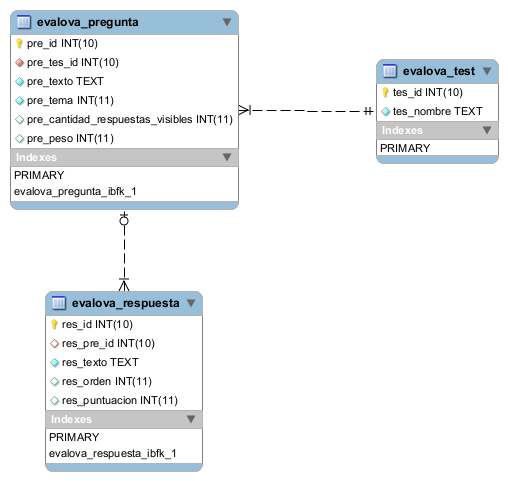
\includegraphics[width=12cm,clip]{Imagenes/SQL_Test.png}
\end{center}
\caption{Modelo entidad-relación del módulo de evaluación}
\label{sql_test}
\end{figure}

La calificación se realiza utilizando una normalización estadística de los pesos de las respuestas de cada pregunta y multiplicándolas por el peso de la respectiva pregunta el cual esta también normalizado entre todas las preguntas del cuestionario, por consiguiente se logran que los cuestionarios sean configurados por el docente de una forma libre.

\clearpage
\begin{center}
 \section{Resultados y pruebas}
\end{center}

Se obtuvo como resultado un objeto virtual de aprendizaje basado en el manejador de contenidos web Drupal diseñado para explicar la teoría del caos desde la perspectiva de la computación evolutiva. Dicha aplicación cuenta con material de estudio dinámico, un módulo de auto-evaluación y un conjunto de aplicaciones que facilitan la comprensión de los conceptos abordados, además de un diseño gráfico agradable y cuenta con internacionalización, ya que esta traducida a los idiomas español, ingles y portugués. Se utilizo Drupal por que con su sistema de manejo de contenidos se logra interoperabilidad, reusabilidad y adaptabilidad, para lograr un crecimiento uniforme llevando a la estandarización de toda la aplicación y permitiendo agregar funcionalidades o características nuevas para alimentar más la aplicación.

Se llevaron a cabo pruebas en que el usuario manejaba la aplicación y calificaba aspectos de ésta como la configuración de colores, los tamaños, la estructura y la usabilidad. De igual manera podían sugerir nuevas funcionalidades o anotar falencias que no estuvieran contempladas en la prueba. La aplicación final es el resultado de implementar la mayor parte de las observaciones y sugerencias realizadas por los usuarios estudiantes y docentes.

La interfaz de la aplicación se realizo teniendo en cuenta cuestiones tales como navegabilidad, interactividad, usabilidad y arquitectura de la información, esta compuesta principalmente por tres bloques ( véase figura \ref{bloques} ):

\begin{figure}[h] 
\begin{center}
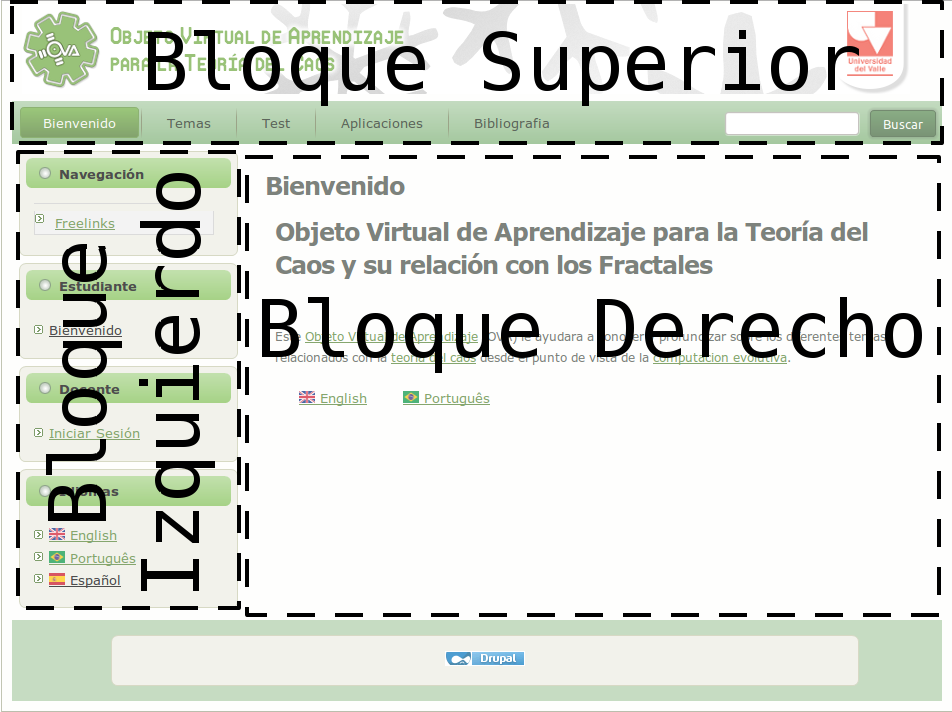
\includegraphics[width=10cm,clip]{Imagenes/bloques.png}
\end{center}
\caption{Bloques principales de la interfaz}
\label{bloques}
\end{figure}

\begin{itemize}
 \item Un bloque superior donde se encuentra el logo y el menú superior, por donde se pueden acceder a las diferentes secciones que componen la aplicación y además de un cuadro de búsqueda.
 \item Un bloque izquierdo en el cual se muestran los menús respectivos según la sección que se esté visitando.
 \item Un bloque derecho donde se muestra el contenido principal de acuerdo a la pagina que se este visitando seleccionada por medio de los diferentes menús. Al final de este bloque se da la opción de cambiar el idioma del contenido si esta disponible la traducción.
\end{itemize}



A contunuación se detallarán las secciones de la aplicación en el cuadro \ref{mapa} con una breve descripción y los menús que se encuentran en cada una de ellas, luego se entra en detalle en cada uno de ellos.

%mapa del sitio
 \begin{table}[h]
\centering
\begin{tabular}[htb]{ p{2cm} | p{3.5cm} | p{6.5cm} }
\toprule
\rowcolor[gray]{0.9}Sección & Descripción & Subsecciones (Menús) \\
\midrule
  Bienvenida & Se encuentran los menús principales para el estudiante y el docente  & \begin{itemize}[itemsep=0pt,topsep=-5pt]                                                                                                                                                                                                                                                                                                                                                                                          
% \setlength{\itemsep}{-5pt}
\item Menú Docente                                                                                                                                                                                                                                                                                                                                                                                              
\item Menú Estudiante
\item Idiomas
 \end{itemize}
 \\
\midrule
 Temas & Ingreso a todos los temas en general  & \begin{itemize}[itemsep=0pt,topsep=-5pt] \item Menús del temario  \end{itemize} \\
\midrule
 Test & Ingreso al módulo de evaluación &  \begin{itemize}[itemsep=0pt,topsep=-5pt]                                                                                                                                                                                                                                                                                                                                                                                                
\item Test                                                                                                                                                                                                                                                                                                                                                                           
\item Configuración de test (Docente)
 \end{itemize}
\\
\midrule
 Aplicaciones & Ingreso a las mini-aplicaciones   &  \begin{itemize}[itemsep=0pt,topsep=-5pt]                                                                                                                                                                                                                                                                                                                                                                                 
\item Visualizador de fractales
\item Conjunto de Mandelbrot
 \end{itemize}
 \\ 
\midrule
 Bibliografía & Referencias a más información interesante & \begin{itemize}[itemsep=0pt,topsep=-5pt] \item Bibliografía  \end{itemize} \\ \\
\bottomrule
\end{tabular}
 \caption{Secciones de la aplicación}
 \label{mapa}
 \end{table}

\clearpage
\newpage

\subsection{Pagina inicial}

En la sección de bienvenida se encuentra una información de bienvenida a la aplicación y los menús principales para el estudiante y el docente, donde están las opciones a las cuales ellos pueden acceder y el menú de idiomas el cual permite cambiar el idioma de toda la aplicación. El docente una vez se haya autenticado tiene acceso a mas opciones en la misma aplicación y en las mismas secciones sin necesidad de tener que entrar a opciones confusas, también en la misma presentación creando una familiaridad con la interfaz.

\subsubsection{Roles de usuario}

El objeto virtual de aprendizaje cuenta con un sistema de usuarios y roles, los roles se usan para asignar permisos a grupos de usuarios, los roles existentes en la plataforma son:

\begin{itemize}
  \item {\bf Rol administrador :} Encargado de la gestión de toda la plataforma puede modificar menús, bloques y configuraciones en general mediante formularios versátiles evitando la necesidad de editar código y disminuir posibles errores y la estabilidad del sistema.
    
  \item {\bf Rol docente :} Es un usuario autenticado encargado de la edición de contenido para lo cual cuenta con editor WYSIWYG (What you see is what you get) que le permite una edición de texto enriquecido en la web para una sencilla redacción del contenido, y así se pueda centrar la atención en el diseño y redacción del contenido y no en aspectos técnicos, cumpliendo con uno de los objetivos del objeto virtual de aprendizaje que el usuario final se dedique de lleno a la creación, estructuración y edición del contenido, siendo transparente para él, el proceso de funcionamiento web de la página.

 \item {\bf Rol estudiante :} Es cualquier visitante y que no necesita autenticarse para que la aplicación sea accesible a toda persona interesada, puede recomendar enlaces o bibliografía para que la página se alimente continuamente, estas recomendaciones por defecto no quedan publicadas deben ser autorizadas por el docente para su publicación y automáticamente agregarlo al listado. Puede interactuar con las mini-aplicaciones y profundizar en el contenido del temario.
\end{itemize}

\newpage

\subsubsection{Internacionalización}

En Drupal cada contenido es un nodo que se puede editar mediante un formulario flexible, en este formulario se pueden hacer vinculaciones a otros nodos, lo cual nos permite indicar qué nodo tiene la traducción de otro nodo y el idioma en el que se encuentra, así cada nodo es independiente de los demás sin importar su idioma, lo que permite mayor flexibilidad, en casos que se quiera mostrar algo mas en determinado idioma, o no se quiera mostrar determinado nodo en otros idiomas.

% \clearpage
\subsection{Temas}

Se muestra un menú por cada tema principal en el temario ( véase cuadro \ref{Temario} ), el estudiante puede ingresar a cualquier tema o concepto que esté interesado en profundizar sus conocimientos.

\subsection{Test}

La sección test carga un menú para realizar algunos de los test por parte del estudiante y otro menú para la configuración de estos, aparece automáticamente un test por cada tema principal en la aplicación.  

\clearpage
\newpage
\subsubsection{Módulo de evaluación}

El módulo de evaluación hace parte del conjunto de los módulos de Drupal, el cual tiene su propio modelo de persistencia (véase \ref{sql_test}) y aprovechando la funcionalidad del módulo \textit{PHP filter} que permite la evaluación de fragmentos de código PHP, su implementación está realizada mediante código insertado en paginas de contenido.

\begin{figure}[h] 
\begin{center}
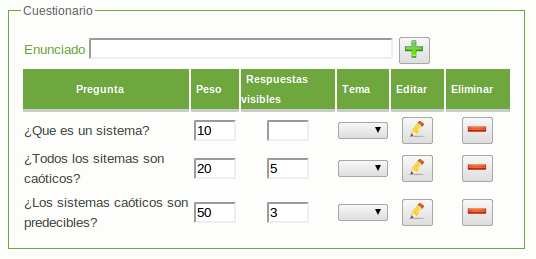
\includegraphics[width=12cm,clip]{Imagenes/config_pregunta.png}
\end{center}
\caption{Interfaz para la configuración de preguntas de un cuestionario}
\label{config_pregunta}
\end{figure}

\begin{figure}[h] 
\begin{center}
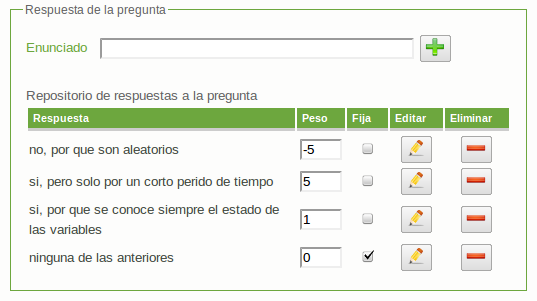
\includegraphics[width=12cm,clip]{Imagenes/config_respuesta.png}
\end{center}
\caption{Interfaz para la configuración de respuestas de un cuestionario}
\label{config_respuesta}
\end{figure}


La vista de configuración del módulo de evaluación es solo visible para el docente en la sección de test, cuenta con una interfaz intuitiva como la mostrada en las figuras \ref{config_pregunta} y \ref{config_respuesta} dando una facilidad de uso para el docente.

\clearpage
\newpage

\subsection{Aplicaciones}

La herramienta cuenta con mini-aplicaciones realizadas basades en el elemento canvas de HTML 5 para que el usuario pueda interactuar y utilizar los conceptos aprendidos para un afinamiento de los conocimientos.

\subsubsection{Visualizador de fractales} 
 
En esta aplicación se puede construir fractales basado en reglas de los sistemas de Lindenmayer. Para su configuración se cuenta con un alfabeto predefinido que está compuesto de cualquier letra mayúscula, el signo más y el signo menos. En el momento de dibujar el sistema cualquier letra mayúscula sera interpretada como un segmento de recta, el signo más indica que se girará en el sentido de las manecillas del reloj tantos grados haya indicado el usuario y el signo menos en sentido contrario. Para dibujar el fractal presiona el respectivo botón y en el cuadro de dibujo se dibujara la primera iteración de la configuración realizada, luego mediante clics del mouse se puede seguir iterando y dibujando la nueva iteración del fractal.
Puedes navegar en dos dimensiones por el fractal. Para desplazarte (mover el fractal), lleva a cabo una de las acciones siguientes:
\begin{itemize}
\item Haz clic y arrastra el mapa.
\item Haz doble clic para iterar el fractal.
\item Pulsa la tecla arriba en el teclado para moverte al Norte.
\item Pulsa la tecla abajo en el teclado para moverte al Sur.
\item Pulsa la tecla derecha en el teclado para moverte al Este.
\item Pulsa la tecla izquierda en el teclado para moverte al Oeste.
\item Para acercar o alejar la imagen, pulsa las teclas + o -. Mueve el cursor sobre una ubicación y utiliza la rueda del ratón para acercarte o alejarte de la ubicación. Para centrar el mapa y acercarte, haz doble clic sobre la ubicación.
\end{itemize}

\begin{figure}[h]
\begin{center}
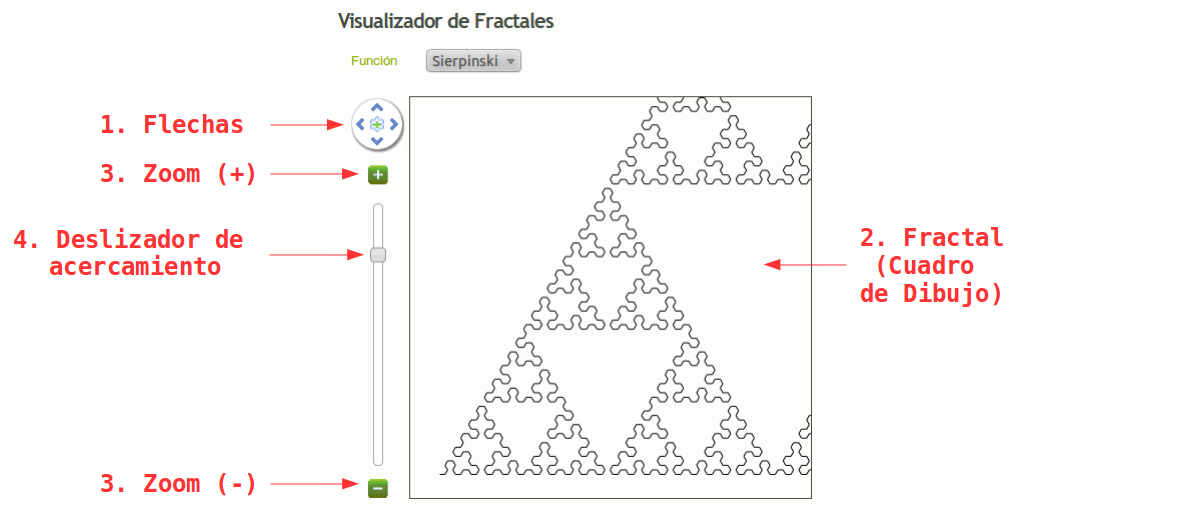
\includegraphics[width=16.5cm,clip]{Imagenes/visualizador.png}
\end{center}
\caption{Interfaz del visualizador de fractales}
\label{visualizador}
\end{figure}

Uso de los controles de navegación

Los controles de navegación se muestran a la izquierda. Los controles de navegación son los siguientes:
\begin{enumerate}
 \item Flechas: haz clic en el botón de flecha adecuado para mover la vista al Norte, Sur, Este u Oeste.
 \item Fractal : haz clic aquí para iterar el fractal.
 \item Zoom: haz clic en + para acercar la imagen del centro del mapa. Haz clic en - para alejarla.
 \item Deslizador de acercamiento: arrástralo arriba o abajo para acercar o alejar la imagen progresivamente.
\end{enumerate}

La aplicación tiene por defecto los fractales de copo de nieve de Koch y el triangulo de Sierpinski y permite agregar nuevas configuraciones por parte de los estudiantes.
\clearpage
\newpage
\subsubsection{Conjunto de Mandelbrot} 
La aplicación del conjunto de Mandelbrot nos muestra un fractal creado por  Benoit Mandelbrot, tomado de un proyecto externo \cite{CanvasMandelbrot}. Este nos permite explorarlo con facilidad y rapidez, entendiendo rápidamente la propiedades de este fractal.

\begin{figure}[h]
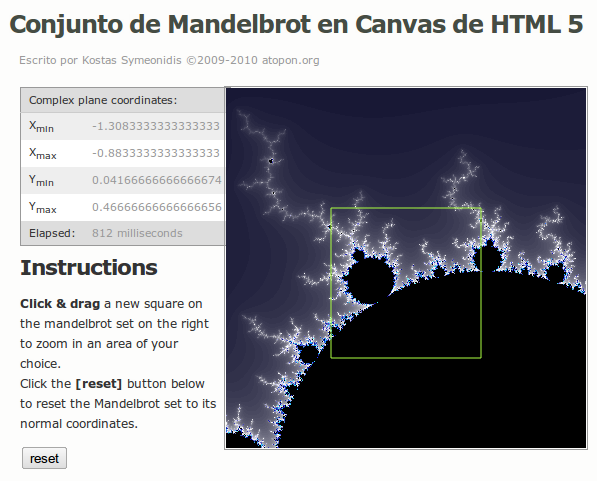
\includegraphics[width=15cm,clip]{Imagenes/mandelbrot.png}
\caption{Conjunto de Mandelbrot en canvas de html5}
\label{mandelbrot_canvas}
\end{figure}

\subsection{Bibliografía}

En esta sección los estudiantes pueden ver diferentes enlaces a otras paginas y pueden recomendar enlaces para que el sitio sea dinámico.
\clearpage
\newpage
\subsection{Pruebas realizadas}

Se diseño una encuesta para medir la usabilidad, facilidad de manejo y comprensión de la herramienta, la cual fue realizada a veinte estudiantes de varios semestres de ingeniería de sistemas, para obtener una variedad con respecto a quienes han cursado la asignatura computación evolutiva y quienes no, además, también fue realizada a estudiantes de otras carreras interesadas como matemáticas y otras ingenierías para valorar el producto no solo como un desarrollo de software sino también como una herramienta útil de aprendizaje para diverso público interesado. \\

\begin{table}[htbp]
\begin{center}
\begin{tabular}{|p{1.6cm}|p{1.8cm}|p{1.8cm}|p{1.8cm}|p{1.8cm}|p{1.8cm}|p{1.8cm}|}
\hline
\textbf{Pregunta} & \multicolumn{ 6}{c|}{\textbf{Respuesta}} \\ \hline
\textbf{1} & \multicolumn{ 6}{c|}{\textbf{Al ingresar a la aplicación, esta le parece :}} \\ \hline
 & \multicolumn{ 2}{c|}{a) Amigable} & \multicolumn{ 2}{c|}{b) Confusa} & \multicolumn{ 2}{c|}{c) Entendible} \\ \hline
 & 16 & 80,00\% & 1 & 5,00\% & 3 & 15,00\% \\ \hline
\textbf{2} & \multicolumn{ 6}{c|}{\textbf{La forma como la aplicación está distribuida como le parece :}} \\ \hline
 & \multicolumn{ 2}{c|}{a) Buena} & \multicolumn{ 2}{c|}{b) Mala} & \multicolumn{ 2}{c|}{c) Regular} \\ \hline
 & 17 & 80,00\% & 1 & 5,00\% & 2 & 10,00\% \\ \hline
\textbf{3} & \multicolumn{ 6}{c|}{\textbf{La internacionalización del sitio y el manejo de varios idiomas es :}} \\ \hline
 & \multicolumn{ 2}{c|}{a) Funcional} & \multicolumn{ 2}{c|}{b) Mala} & \multicolumn{ 2}{c|}{c) Regular} \\ \hline
 & 15 & 75,00\% & 4 & 20,00\% & 1 & 5,00\% \\ \hline
\textbf{4} & \multicolumn{ 6}{c|}{\textbf{La manera de navegar e interactuar con la aplicación le parece :}} \\ \hline
 & \multicolumn{ 2}{c|}{a) Buena} & \multicolumn{ 2}{c|}{b) Mala} & \multicolumn{ 2}{c|}{c) Regular} \\ \hline
 & 16 & 80,00\% & 0 & 0,00\% & 4 & 20,00\% \\ \hline
\textbf{5} & \multicolumn{ 6}{c|}{\textbf{Los nombres de los campos en la aplicación le parece que son:}} \\ \hline
 & \multicolumn{ 2}{c|}{a) Precisos} & \multicolumn{ 2}{c|}{b) Confusos} & \multicolumn{ 2}{c|}{c) No están acorde} \\ \hline
 & 15 & 75,00\% & 4 & 20,00\% & 1 & 5,00\% \\ \hline
\textbf{6} & \multicolumn{ 6}{c|}{\textbf{Los colores utilizados le parecen :}} \\ \hline
 & \multicolumn{ 2}{c|}{a) Agradables} & \multicolumn{ 2}{c|}{b) Poco Agradables} & \multicolumn{ 2}{c|}{c) Nada Agradables} \\ \hline
 & 15 & 75,00\% & 5 & 25,00\% & 0 & 0,00\% \\ \hline
\textbf{7} & \multicolumn{ 6}{c|}{\textbf{ La aplicación le parece interactiva :}} \\ \hline
 & \multicolumn{ 2}{c|}{a) Si} & \multicolumn{ 2}{c|}{b) No} & \multicolumn{ 2}{c|}{c) Poco} \\ \hline
 & 9 & 45,00\% & 4 & 20,00\% & 7 & 35,00\% \\ \hline
\textbf{8} & \multicolumn{ 6}{c|}{\textbf{La interfaz cumple con sus expectativas :}} \\ \hline
 & \multicolumn{ 2}{c|}{a) Si} & \multicolumn{ 2}{c|}{b) No} & \multicolumn{ 2}{c|}{- -} \\ \hline
 & 19 & 95,00\% & 1 & 5,00\% & - - & - - \\ \hline
\textbf{9} & \multicolumn{ 6}{c|}{\textbf{El contenido de la aplicación es suficiente para su aprendizaje :}} \\ \hline
 & \multicolumn{ 2}{c|}{a) Si} & \multicolumn{ 2}{c|}{b) No} & \multicolumn{ 2}{c|}{c) Solo en parte} \\ \hline
 & 13 & 65,00\% & 2 & 10,00\% & 5 & 25,00\% \\ \hline
\textbf{10} & \multicolumn{ 6}{c|}{\textbf{Cómo le parece la forma en que se presenta la información :}} \\ \hline
 & \multicolumn{ 2}{c|}{a) Adecuada} & \multicolumn{ 2}{c|}{b) Difícil de entender} & \multicolumn{ 2}{c|}{- -} \\ \hline
 & 17 & 85,00\% & 3 & 15,00\% & - - & - - \\ \hline
\textbf{11} & \multicolumn{ 6}{c|}{\textbf{El modo en el que se editan los contenidos es :}} \\ \hline
 & \multicolumn{ 2}{c|}{a) Sencilla} & \multicolumn{ 2}{c|}{b) Poco Intuitiva} & \multicolumn{ 2}{c|}{c) Complicada} \\ \hline
 & 5 & 25,00\% & 11 & 55,00\% & 4 & 20,00\% \\ \hline
\textbf{12} & \multicolumn{ 6}{c|}{\textbf{La forma de evaluación es :}} \\ \hline
 & \multicolumn{ 2}{c|}{a) Sencilla} & \multicolumn{ 2}{c|}{b) Poco Intuitiva} & \multicolumn{ 2}{c|}{c) Complicada} \\ \hline
 & 17 & 85,00\% & 3 & 15,00\% & 0 & 0,00\% \\ \hline
\textbf{13} & \multicolumn{ 6}{c|}{\textbf{ Las mini-aplicaciones son :}} \\ \hline
 & \multicolumn{ 2}{c|}{a) Sencilla} & \multicolumn{ 2}{c|}{b) Poco Intuitiva} & \multicolumn{ 2}{c|}{c) Complicada} \\ \hline
 & 3 & 15,00\% & 12 & 60,00\% & 5 & 25,00\% \\ \hline
\textbf{14} & \multicolumn{ 6}{c|}{\textbf{La cantidad de idiomas en la aplicación le parece:}} \\ \hline
 & \multicolumn{ 2}{c|}{a) Acorde} & \multicolumn{ 2}{c|}{b) Innecesaria} & \multicolumn{ 2}{c|}{c) Distractora} \\ \hline
 & 9 & 45,00\% & 3 & 15,00\% & 8 & 40,00\% \\ \hline
\end{tabular}
\end{center}
\caption{Resultados de las encuestas}
\label{encuesta}
\end{table}


Después de analizar los resultados de las encuestas. Se obtuvo que el diseño gráfico de la aplicación en cuanto a forma y colores es agradable a la vista, y sobresale por mantener una interfaz coherente y bien definida. \\

Se comprobó que el contenido temático de la aplicación es explicado de una forma coherente y el manejo de los temas es abordado de una forma secuencial, se recalco la oportuna explicación de términos base para un mejor entendimiento y que dicha explicación se encuentra presente de una manera de rápido acceso, abriendo la oportunidad del uso de la aplicación a más personas. \\

Se encontraron deficiencias en la usabilidad de las mini-aplicaciones relacionadas con los fractales, ya que sin un apropiado entendimiento previo de lo que se está visualizando se dificulta la interacción y llega a confundir fácilmente al usuario. Mas sin embargo, la aplicación de evaluación tanto en la forma como un docente configura los cuestionarios, como en la forma en la que los estudiantes contestan tales cuestionarios se realiza de manera intuitiva y la visualización de los resultados le da al estudiante realmente un indicio del nivel de conocimiento que tiene. \\

El uso de varios idiomas e internacionalización de la aplicación se realiza de forma sencilla y es de gran utilidad pero puede llegar a desenfocar la atención del estudiante y así distraerlo fácilmente. \\

El editor de textos enriquecido produce varias confusiones y problemas y muchas veces es necesaria ayuda adicional para lograr ediciones que se suponen son sencillas, y no es muy intuitivo para el uso de diversas herramientas como posicionamiento de tablas e imágenes. \\

 \clearpage
 \newpage
\subsection{Evaluación del objeto virtual de aprendizaje}
En esta sección se analiza de forma critica el trabajo propuesto teniendo en cuenta los criterios de diseño, los preceptos de los objetos virtuales de aprendizaje y los elementos del sistema de gestión de aprendizaje.

\subsubsection{Criterios de diseño}
Según el ministerio de educación nacional\cite{Roldan05}, un objeto virtual de aprendizaje tiene cinco criterios que deben manejar, en el trabajo propuesto estos conceptos están tratados de la siguiente manera:

\begin{itemize}
 \item Atemporalidad : La teoría del caos es un tema que tuvo auge en la segunda mitad del siglo XX, por lo que en el área de las matemáticas es un tema novedoso. Los fundamentos matemáticos que se explican en la aplicación no tienen muchos cambios y pueden perdurar en el tiempo, mas sin embargo las aplicaciones se pueden seguir mejorando y el uso de la teoría del caos y los fractales en la vida real es un tema de investigación que se renueva constantemente.
 \item Didáctica : El objeto responde correctamente al publico a que va dirigido la aplicación y tiene definidos la forma de enseñanza y lo que enseña.
 \item Usabilidad : El objeto y sus componentes fueron diseñados de una forma en la que el estudiante no se pueda distraer con facilidad y sea lo suficientemente interactiva para que el estudiante adquiera los conocimientos de una forma agradable y entretenida.
 \item Interacción :  El objeto esta diseñado para que el estudiante entienda los fundamentos de la teoría del caos, e incentivar una profundización de ellos que sera eventualmente realizada por parte del docente.
 \item Accesibilidad : Uno de los criterios importantes es que este abierto al publico en general, y no tenga ningún tipo de restricción, por lo tanto cualquier persona interesada puede acceder a la aplicación. 
\end{itemize}
 
\subsubsection{Preceptos de los objetos virtuales de aprendizaje}

En aspectos como reusabilidad, interoperabilidad, mantenibilidad entre otros la aplicación es débil, ya que no se utilizo ningún estándar o colección de estándares de enseñanza virtual como SCORM, lo que no permite relacionarse fácilmente con otros objetos virtuales.

\subsubsection{Elementos del sistema de gestión de aprendizaje}
Dado que el trabajo presentado no tiene como objetivo reemplazar la metodología que el docente este utilizando actualmente, si no dar un apoyo al docente e ir adaptando el uso de tecnologías a la metodología utilizada. Las herramientas comunes en los sistemas de gestión de aprendizaje fueron trabajadas de manera somera para que dicha adaptación se realice de manera gradual. \\

Como herramientas de comunicación se cuestiono la idea de implementar foros, un blog, o algún sistema parecido, pero se llego a la conclusión de que por el momento un sistema parecido es innecesario, ya que una explicación mas profunda del tema se da mejor de manera personal y a la vez el docente tiene una manera de ir midiendo el entendimiento en los alumnos y el interés por el tema que haya generado el objeto virtual. Pero se incluyo la sección de bibliografía donde los interesados pueden compartir enlaces. \\

Como herramientas de gestión de usuarios y cursos, se decidió que no era necesario el manejo de usuarios, ya que se desea que el sistema este abierto al publico en general y por lo tanto que no requiera algún tipo de registro o estar matriculado en alguna clase. Y como manejo de cursos, tampoco es necesario ya que el contenido de la aplicación es solo un tema de un curso, esta parte seria necesaria en un futuro cuando se unifique con mas temas relacionados. \\

Como herramienta de almacenamiento de información, es el aspecto en el que la aplicación es mas completa gracias a la ayuda del sistema de manejo de contenidos, ya que permite editar de manera sencilla cualquier texto presentado. \\

\subsubsection{Comparación con otros objetos virtuales de aprendizaje}

Se realiza una comparación con los objetos mencionados en el capítulo 3 con el objeto presentado en este trabajo, en los aspectos detallados en ese capitulo y los de la sección anterior.

\begin{table}[htbp]

\begin{center}
\begin{tabular}{|p{2.5cm}|p{2.5cm}|p{2.8cm}|p{3.2cm}|p{2cm}|}
\hline
\multicolumn{1}{|c|}{\textbf{Características}} & \textbf{OVA Caos} & OVA The Chemistry Collective & OVA PhET Interactive simulations & OVA Parques Naturales \\ \hline
Atemporalidad & El tema es novedoso y puede tener varios cambios & El tema y las actividades no pierden vigencia en el tiempo & El tema y las actividades no pierden vigencia en el tiempo & El tema es interesante y genera conciencia \\ \hline
Didáctica & El proceso de enseñanza se realiza con guía del docente & El proceso de enseñanza se realiza con guía del docente & Intentan imponer una ayuda autodidacta & Esta enfocado al publico en general \\ \hline
Usabilidad & Requiere conocimientos en el tema & Requiere conocimientos en el tema & Son simulaciones fáciles de entender & Es fácil de usar \\ \hline
Interacción & Genera curiosidad en algunas personas & Es entretenida, pero puede ser enredada & Tiene elementos de la vida real, por lo que genera bastante experiencias & Genera conciencia ambiental \\ \hline
Accesibilidad & Se puede acceder fácilmente & Requiere software extra & Requiere software extra & Se puede acceder fácilmente \\ \hline
Comunicación & Permite intercambiar bibliografía & Contacto por correo electrónico & Contacto por correo electrónico & No Aplica \\ \hline
Usuarios & Tiene acceso a docentes para gestión del contenido y traducciones & En colaboración con otras paginas & Tiene acceso a estudiantes y docentes  para traducciones y contacto & No Aplica \\ \hline
Archivos & Permite almacenar diversos tipos de archivo & No posee & No posee, solo tiene las simulaciones & No Aplica \\ \hline
\end{tabular}
\end{center}
\caption{Comparativa entre objetos virtuales de aprendizaje}
\label{comparacion}
\end{table}


\clearpage
\begin{center}
 \section{Conclusiones}
\end{center}

La realización del proyecto permitió obtener muy valiosas conclusiones en las áreas de matemática, computación evolutiva y pedagogía como también de las herramientas y tecnologías usadas para la realización de la aplicación. Asimismo, surgieron ideas y motivaciones para la expansión de funcionalidades de la aplicación, las cuales por el alcance y tiempo del proyecto no fueron abordadas. A continuación se verán las conclusiones obtenidas y los trabajos futuros propuestos.\\

  \subsection{Conclusiones}
\begin{itemize}
 \item  La complejidad de la geometría fractal y el caos, los insuficientes conocimientos de matemáticas y la falta de formación previa son los principales obstáculos para el proceso de aprendizaje.
 \item Los objetos virtuales de aprendizaje tienen diversas posibilidades de uso, desde ayudar a la motivación y concentración de los estudiantes, hasta ser el soporte de una clase completa en sus distintos momentos. Resultan una herramienta atractiva para los estudiantes, por el formato digital y los niveles de interactividad que tienen. Pueden ser utilizados de manera individual o colectiva, con o sin mediación del docente. A partir de estas y otras características, tienen grandes posibilidades de contribuir a generar aprendizajes de calidad en los estudiantes.  
 \item La creación de recursos digitales como los objetos virtuales de aprendizaje hace que la labor del docente se redimensione, ya que éste debe poseer las competencias suficientes en el uso de herramientas informáticas unidas a su habilidad para crear espacios en donde el estudiante encuentre escenarios propicios para su aprendizaje.
\item Se ha visto que el uso de estilos de aprendizaje como estrategia durante el proceso de enseñanza crea un impacto positivo en la forma que el estudiante aprende; por lo tanto, la utilización de objetos multimediales que representen las características de dichos estilos generan un medio más versátil para la asimilación de información por parte del estudiante.
 \item Las evaluaciones en una plataforma virtual muchas veces se realizan de una forma general, pueden llegan a ser predecibles y aburridas para los estudiantes, por lo que crear algo de aleatoriedad puede ayudar a mejorar la autoevaluación.  
\end{itemize}

  \subsection{Trabajos futuros}
\begin{itemize}
\item Incorporar la aplicación a un banco de objetos de la asignatura computación evolutiva, y relacionarse con otros temas.
\item Agregar mas formas de evaluación, de manera que imponga retos a los estudiantes.
\item Realizar mas contenido multimedia como vídeos, imágenes, animaciones, gráficas que muestren de una manera mas detallada características de temas específicos.
\item Cubrir diversos estilos de aprendizaje, para de esta manera lograr una experiencia enriquecedora para varias formas de estudio de los alumnos.
\item Incluir mini-aplicaciones que muestren usos actuales de la teoría de la caos, principalmente enfocados en las ciencias de la computación.
\item Incluir gráficas interactivas que muestren la forma como interactúan diferentes ecuaciones caóticas.
\item Agregar mas contenidos e información desde el punto de términos matemáticos en cuanto a sistemas dinámicos y resolución de estos.
\end{itemize}
 
% \clearpage
\clearpage

\bibliography{Bibliografia.bib}
\end{document}